\RequirePackage[2020-02-02]{latexrelease}
\documentclass[12pt,onecolumn,aps,prb,preprint]{revtex4}   % style for Physical Review B and AJP are similar
\usepackage{amsmath}    % need for subequations
\usepackage{amssymb}
\usepackage{graphicx}
\usepackage{subfigure}
\usepackage{svg}
\usepackage{listings}
\newcommand{\dprime}{{\prime \prime}}
\newcommand{\beao}{\begin{eqnarray}}
\newcommand{\eeao}{\end{eqnarray}}
\newcommand{\mypm}{\mathbin{\mathpalette\@mypm\relax}}

\begin{document}
\begin{abstract}
{
    Mechanising Islamic calligraphy is a challenging job that demands research both in the process of digitization of existing art and the creation of new scripts. This research first yields a novel innovation in the conventional bezier spline curves to use them to effectively answer the artistic requirements of copying or creating broad-edge calligraphy scripts and then mathematically compares the output with the original specimens. Since these twisting spline curves also claim to bridge the gap between digital script data and a robotic manipulator that needs machine data to start moving, a robotic simulator is also discussed. The robustness of the simulator and its efficiency with the twisting bezier splines is demonstrated. The research also proposes a novel method to represent, design and solve robotic manipulators. It is believed that this research can be considered a major milestone in mechanising Islamic calligraphy given more attention and resources.
}
\end{abstract}

\maketitle
\tableofcontents
\section{Introduction}
{
    Islamic calligraphy is an art having a history that dates back to the seventh century \cite{bib01, bib02}. It has witnessed many evolutionary stages \cite{bib02, bib03} and has been used by artists speaking several different languages \cite{bib04} and sharing uncommon biographies \cite{bib05,bib06,bib07,bib08}. Unfortunately though, the industrial age and the advent of technology has not spared this beautiful art when it claims to provide better alternatives for almost everything related to human beings. Discovery of new facets of calligraphy aside, with the prevalence of modern technologies and resulting lack of expertise in this domain, the very existence of Islamic calligraphy now faces a serious threat. Public buildings and infrastructure that once used to be a showcase for the most laudable artists of the time have turned in-to museums; awaiting to be wiped away slowly with each round of the monsoon and every splash of the ocean’s waves.

    Potentially, we can use robotic dexterity to help us in this domain. Industrial robots have already been used outside the industry to do unorthodox tasks \cite{bib09, bib10,bib11,bib12} and they can surely uplift this art as well. At the very least, they can be employed in restoration and replication of existing calligraphy work \cite{bib13}. In other words, they can be used as printers, or rather one may say, “painters” that give an extra hand to the calligraphy artists to open up a new dimension of art that can not only revamp the existing calligraphy sites but also create new ones.

     Mechanized/robotic drawing of the Islamic calligraphy scripts requires not just the ink-mark information but also the information about the tool movement \cite{bib03}. Specially, using a flexible broad edge brush instead of a solid round tip pen and all that to draw on un-even surfaces, makes the job extremely special indeed. A robot needs to take special care about the orientation and downwards force of the tool as well.

    In a nutshell, the main problem can be divided in two major sections. First, transforming the printed scripts into machine data and second, recreating the scripts using a robotic end effector.
    
    To solve the first part, instead of doing image processing, we propose a new way of transforming the existing scripts into machine data; the “Rotating/twisting Bezier Spline Curves”, or simply, ``Twisting Bezier Splines''. The idea is to bring real artists in the process. For the new scheme to be fully tested, a fully featured graphical spline editor and analyzer would also be needed. The tool was tested and tuned with the help of multiple real-world calligraphers.

    To answer the second part of the problem, we discuss the working of a robotic simulator written specifically for the research. The usage, working principle and some benchmarks of the simulator are also shared.
    
    The thesis is divided in seven sections. After the introduction, section \ref{Chapter:Problem Statement} states the problem and proposes a solution and discusses the challenges that need to be overcome. Discussing the detail of the proposed solutions, section \ref{Chapter:Twisting Splines} discusses the principal, working and testing of twisting bezier splines. In section \ref{Chapter:RoboticManipulator} we discuss the modelling of the robotic manipulator used in the research. Section \ref{Chapter:Drogon} and \ref{Chapter:Gregor} discuss the software tools written specifically for the research. We finally conclude in Section \ref{Chapter:Conclusion}.
} 
\section{Understanding the Research Problem}\label{Chapter:Problem Statement}
{
    \subsection{The Problem Statement}
    {
        The main problem is to devise a solution to use a robotic manipulator with a broad edge tool to create and copy Islamic calligraphy specimens. This problem can be divided in four main questions:
        \begin{itemize}
          \item How to copy and create broad-edge scripts in the computer?
          \item How to format the data in digital format to include most of the script information?
          \item How to convert the digital data into machine data to be used with actual manipulators?
          \item How accurate and robust is the proposed solution.
        \end{itemize}

        The first task would be to study the existing digital forms of Islamic calligraphy which are mainly based on glyphs and splines that form digital computer fonts. They carry the least information to reproduce the final ink-marks of the script. They don’t carry information about the machine movement. Conventional bezier splines could also solve the problem if they could either be translated into machine data or could somehow contain machine data within in the first place. This new method then needs to be tested and characterised. This is why a simulation solution would also be needed.

    }
    \subsection{The Proposed Solution}
    {
        As we discuss in section \ref{Chapter:Twisting Splines}, the first three questions of the research can be directly answered by one innovation in the conventional bezier splines. We discuss in detail how the twisting splines work but the main idea is to include a human artist in the process. The artist is given a computer interface that mimics a broad edge tool in the same fashion similar to most vector graphics editors that work well for round tip pens. The main strength of the innovation lies in the fact that though the artist may be oblivious to what they are actually producing, they actually are also feeding direct machine data information in the spline. The output is vector data; sum of a number of continuous step functions and can be considered directly as the end effector movement data.

        Once an editor for such splines is ready, the main challenge would be the characterization and testing of the proposed technique. Section \ref{Chapter:Twisting Splines} also shares some results and benchmarks of the twisting splines.

        To verify how well the splines work with a real manipulator, a $6$ DoF robotic manipulator would be needed. Section \ref{Chapter:Drogon} discusses such a simulator written specifically to test the splines. We can use the graphical and programmatic interface of the simulator to test and quantitatively analyze the rotating bezier splines with different configurations of a robot.
    }
}

\section{Rotating/Twisting Bezier Splines}\label{Chapter:Twisting Splines}

    \subsection{Introduction}
    The first part of the main problem is extracting digital machine data from the existing calligraphy specimens.  Conventionally, image processing is being used [cite?] to extract data that can be used to create machine data. We, however, propose a difference; no matter how strong and robust image processing gets, we propose that there is no alternative to the minor details only a real artist can observe and recreate. So a solution is needed that fulfils the technical needs as well as the artistic demands.
    

    \subsection{Digital Script Data}

    An important question while the modeling the calligraphy scripts is the choice of a digital data format that will hold the extracted script data. One potential answer to this question involves using the existing digital calligraphy fonts. There are, however, two critical issues involved with this scheme; one is the need of an algorithm that will convert the font data to robot movement data and the other is the lack of a font variety. Additionally, working with fonts leaves a narrow space of modifying the scripts to look like artistic scriptures. This is the primary reason we must not use the existing digital fonts.

    Keeping in mind the gaps left by the digital font, another solution to this problem is in the discovery of a new way to unify ink-mark information of digital Islamic script and tool movement performed by the artist. Making a mathematical model to learn the drawing tool information just from the printed text is quite a complex job. Instead, only if we could form a way an artist can give digital input, this problem can be overcome.

    This is where the twisting Bezier splines come into play. We add a twist/rotation handle in the conventional Bezier spline [ref] curves and that is it. Another question however arises: Let alone a Twisting Bezier spline, what is a (conventional) Bezier spline curve in the first place?

    \subsection{Mathematical Model of a Rotating Bezier Spline}
    \subsubsection{The Conventional Bezier Spline}
        To describe how twisting splines work, lets first look into the working principle of a conventional Bezier spline. Figure \ref{Fig:RotatingBezierSplines} shows an illustration of a spline path made up of several sub curves. Each curve section is only partly independent of the other. Figure \ref{Fig:RotatingBezierSplines}  (a) shows the final shape of the curve without any construction elements. In Figure \ref{Fig:RotatingBezierSplines} (b), we explode different sections of the curve into smaller elements and show how they fit together to form the complete spline. There five sections in this curve labeled $1$ through $5$. Figure \ref{Fig:RotatingBezierSplines} (c) shows an assembled form of these five sections. It also shows, what are called, anchors and construction handles. The anchor is the point that sits at the terminals of two adjacent curve sections. For instance, Anchor point $A$  is connecting the sections $1$ and $2$. Like all the other anchors, this angle also has two handles, $H_1$ and $H_2$, connected through a straight line passing through the anchor. The length of each handles, $\overline{AH_1}$  and $\overline{AH_2}$ on both sides of the anchor define the shape of the curve section on their respective side where as the orientation of line connecting both handles contributes to the shape on both the curve sections. This is how both section become partly independent. For instance, handle $\overline{AH_1}$ contributes to the shape of curve segment $1$ and $\overline{AH_1}$ to section $2$.


        \begin{figure}
          \centering
          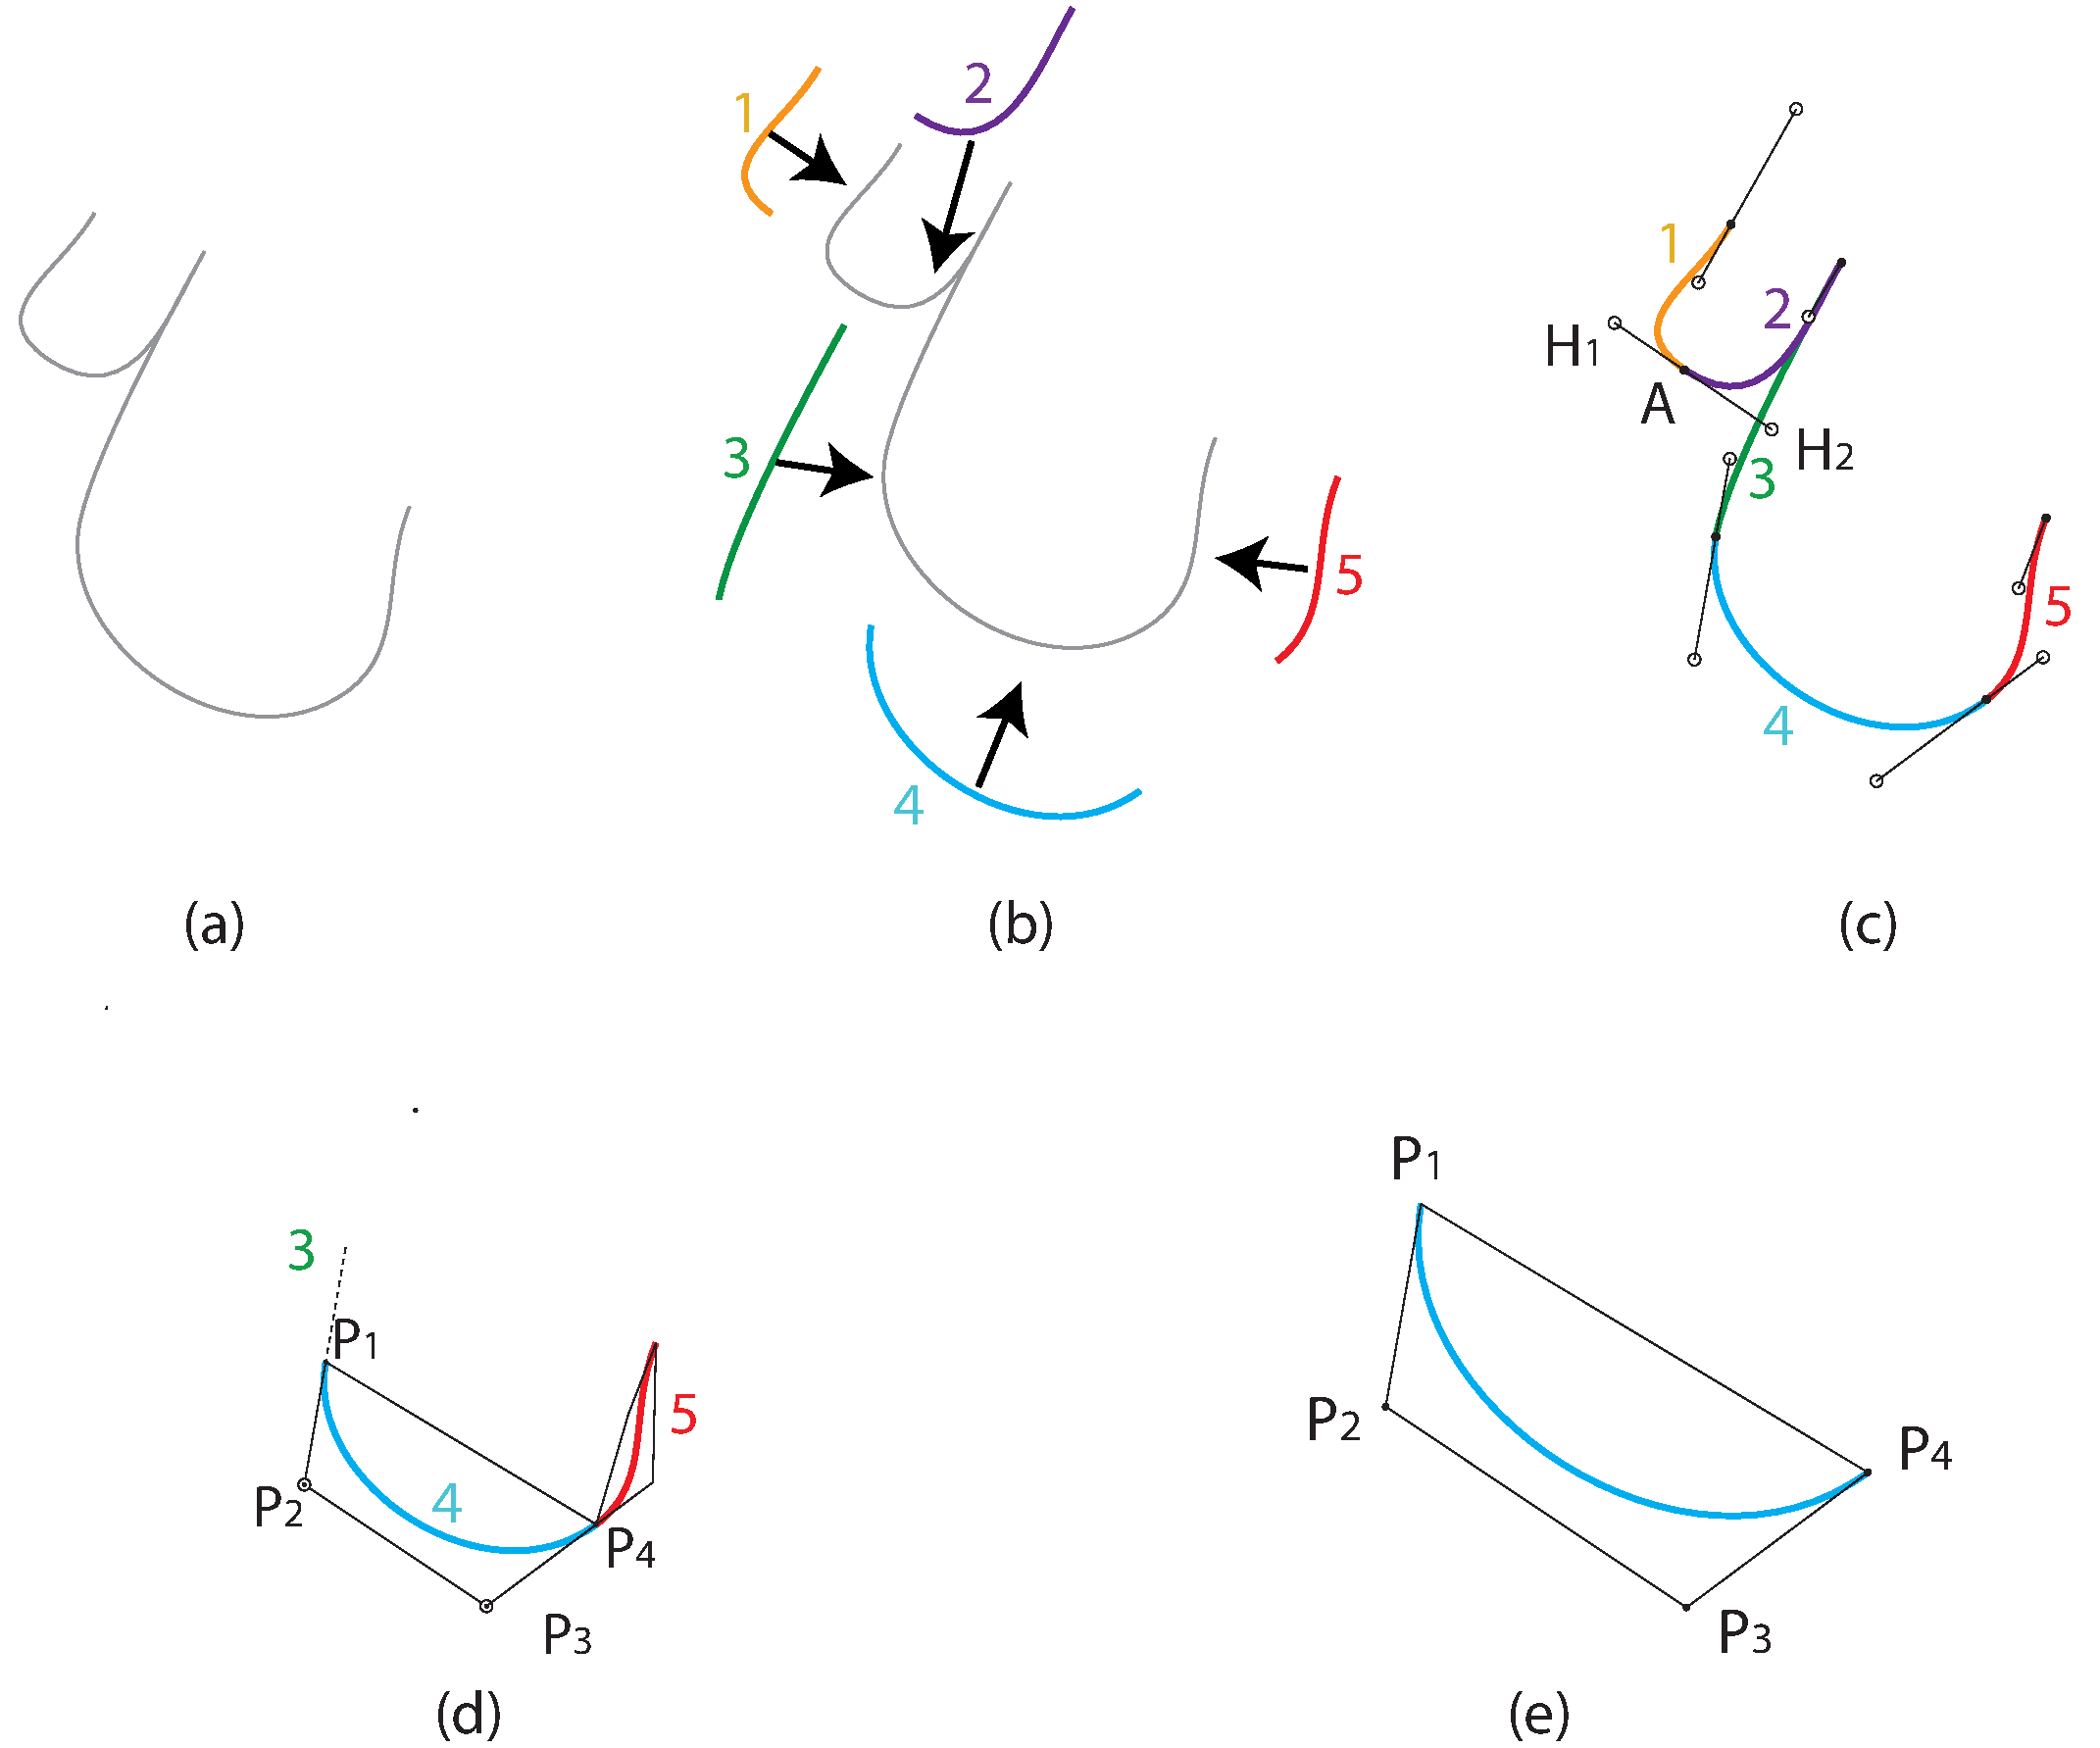
\includegraphics[width=0.9\textwidth]{BezierSplineCurve.pdf}
          \caption{An illustration showing the construction of Bezier Spline Curve. (a) A sample of a Bezier spline path (b) an exploded view of inner curves of the Bezier spline path (c) Handles that control the shape of the two adjacent sub curves (d) and (e) Construction polygon of the sub curve.
          } \label{Fig:RotatingBezierSplines}
        \end{figure}

        Now, it may look like the shapes defined in this way are pretty organic but in fact, the whole shape is defined by simple mathematical equations. Figure \ref{Fig:RotatingBezierSplines} (d) focuses on section $4$ and $5$ of the curve and also shows a polygon defined by the points $P_1$, $P_2$, $P_3$ and  $P_4$. It must be noted that the points $P_1$ and $P_4$ of this polygon are also the anchor point between sections $3$, $4$ and $5$. Take section $4$ for example here. The polygon mathematically defines the complete shape of this polygon. If $P_spline$ is point on the section $4$, with coordinates $x$ and $y$ in a cartesian plane with some origin, it is defined by the following equation.
         \begin{equation}
         P_spline$$=$$P_b×f+P_a×(1 -f)
         \end{equation}
where,
\begin{equation}
P_a=P_23×f+P_12×(1 -f)
\end{equation}
and
\begin{equation}
P_b=P_34×f+P_23×(1 -f)
\end{equation}
where,
\begin{equation}
P_12=P_2×f+P_1×(1 -f)
P_23=P_3×f+P_2×(1 -f)
\end{equation}
and
\begin{equation}
P_34=P_4×f+P_3×(1 -f)
\end{equation}
for an $f$ in the range $[0, 1]$.

It can also be proved that the side segments of the polygon $\overline{P_1 P_2}$ and $\overline{P_3 P_4}$ are tangent to the curve at the point the meet it at $P_1$ and $P_4$ respectively.


\subsubsection{Twist/Rotation Handle}
    On top of the conventional Bezier splines, that work around anchor points that have curvature handles, we add a “Rotation”/”Twist” handle in the anchor and a thickness parameter to the whole curve. A rotation handle is like the curvature handle discussed earlier, except it does not have any effect on the shape of the curve. The thickness parameter defines the size of a flat line centered on $P_spline$ and sweeping on it. The orientation of this sweeping line is the same as the angle between the twist handle and the respective anchor. See Figure 2 (a) that shows rotation handles added in the example under discussion. It must be noted that the curvature of the spline remains the same after adding twist handles that are lying horizontally yet. We then add thickness to the curve in Figure 2 (b). The resulting curve may look a little out of order but it is normal. This is because the rotation handles are lying on their default position. The twist handles may be given some length but it is insignificant since the twist of the curve will only take the value of the angle the handle subtends about the anchor.

    In simpler words, it’s similar to sweeping a pen centered on the actual spline while twisting it uniformly and continuously about its own axis according to the equation
    \begin{equation}
    \theta_twist$$=$$\theta_A  (1-f)+ \theta_B
    \end{equation}
    where $f$ is the same factor that was used to define $P_spline$ and $\theta_A$ and $\theta_B$ are the angles between the first and the second anchor and their rotation handles respectively. It may be noted that since each anchor is connecting two adjacent sub curves, the ending angle of the sweeping line at the end of the first curve is always the same at the beginning of the later. This visually hides the transition of the twisting curve from one sub curve to the other.

    It must also be noted that the angle of rotation handle cannot be constrained in a $2\pi$ domain. Instead, it is completely unbounded, and the sweeping pen may actually take multiple turns both clockwise and anticlockwise while moving on a single curve section as well as the whole curve. When the idea of the twisting splines was first conceived, it wasn’t envisaged that the angle had to be taken like in this scheme. Special care had to be taken in order to graphically read a continuous angle from the user.

    See Table 1 in Appendix which compiles the rectangular coordinates of all the anchors of the rotating bezier spline shown in discussed in this example. Also, see code snippet 1 in appendix which shows the contents of a file that can be used to recreate the spline. In chapter 3, we will discuss “Gregor”, the tool that uses this data to save the created splines.

\subsection{Conversion of Existing Calligraphy Artwork}
Instead of using image processing to try to extract data from existing scans and photographs of the artworks, using rotating Bezier splines we can now include the artists in the process. Just like any other computer-based graphics design application, either we can write a rotating Bezier splines curve editor plugin for an existing open-source application like GIMP [14] or Inkscape [15]. Unfortunately, the later is not a suitable option because the support for the plugins and extensions for both of these poplar software only lets the developer work with the image saving and processing, they don’t let us play with the behavior of the workspace which would be needed to convert the conventional spline tool into a rotating Bezier spline editor. It can still be done by modifying the source code and building the applications from the scratch.

With the second option not viable anymore, we are left with only one option. Writing our own tool to create, modify, save, and reload rotating Bezier splines. Like any other application, for it to be called a “Software”, we also develop some comprehensive documentation discussing the working and behavior of the tool. Although we will discuss in detail about the tool in chapter 3, the fundamental problems it must solve are

\begin{itemize}
\item easy to use interface
\item converting the existing photos to digital form and,
\item generating machine data that that encapsulates the pen rotation information along with other positional and speed information.
\end{itemize}

Keeping in view these requirements we created “Gregor”, the first tool to edit, modify and create rotating Bezier splines. It will be discussed in detail in later chapters

\subsection{Machine Data Generation}
The rotating spline curves are themselves an emulated ink-mark of a broad edge marking tool. This is the reason extracting machine data and even G-codes from them becomes natural. If the flat side of the tool is assumed to be entirely touching the writing surface, the minimum information required to draw a stroke trickles down to the line on which the pen must move and the twist of the pen in world coordinates. This is exactly the rotation Bezier splines can contain once an artist has drawn them on the computer screen. In other words, to call the rotation Bezier splines the machine data, the following assumptions must be made:
\begin{itemize}
	\item The flat tip of a broad edge tool is always completely touching the drawing area.
	\item The inclination of the pen with respect to the drawing area or with respect to the direction of the drawing is either normal or always fixed at an angle and is set by the machine.
	\item To produce thinner strokes, another spline will be used. This means that the machine would have to use multiple tools for such splines.
	\item The axial pressure the pen inserts on the drawing board while drawing is also fixed and the is set by the machine.
\end{itemize}

It is now obvious that to remove the limitations of fixed angles and pressure values, one can add more handles similar to the rotation handle. A set of by directional inclination handles can be added right away with a three-dimensional pen position visualizer to assist the artist determine what angle they want to keep the pen at while drawing a specific stroke. The pressure angle, however, would not be recommended without interfacing some hardware that lets artist feel the pen pressure in real time before setting a handle value. This can be done using a pressure sensitive digital pen or writing tablets [16-18].
There is more detail on how the spline data is converted into machine data in the coming chapters.

\subsection{Characterization}
An important aspect of fabricating a new technique is measuring how well it performs in different usage scenarios. The problem is, in terms of arts, not every mistake the technique makes can be regarded as an issue. Developing a metrics for judging the artistic quality of a calligraphy specimen produced by the Bezier or rotating Bezier splines is altogether a separate discussion and out of scope of this project. However, there are some aspects that we have tried to measure that gives us some idea how effective the rotating Bezier splines can be.

\subsection{Supported Scripts}
The mainline scripts are not necessarily as mathematical as the model of the rotating Bezier splines. Especially, if the artists start to utilize their writing tool in unique ways to extract some unique value from the scripts they create, forming a mathematical model becomes practically impossible. However, since it would be an artist who will be creating and tracing scripts on the screen of a computer, it was safe to claim that given the similarity of the emulation, rotating Bezier splines can be used to produce any script that is written with broad edge tools. However, these are some limitations with this statement:

\begin{itemize}
\item If the tool changes thickness during a stroke (like a flexible brush), the best alternate to achieve a similar appearance of the script would be to use multiple splines with multiple thicknesses that overlap each other in a gradual manner.
\item Although the rotating splines have a defined tool width, the still assume the tool to infinitely thin on the other side, more like a narrow line. This makes negligible but still some difference when the virtual tool is replaced with an actual tool. One way to overcome this issue would to come up with another rendering algorithm that also asks for the missing information. This has been discussed in later chapters when we suggest some other improvements in the overall project.
\end{itemize}
With these assumptions in mind, the “Gregor” was coded.
\subsubsection{Coverage}
To benchmark the performance and accuracy  of rotating bezier splines, some test results are presented here. These values are produced by comparing high resolution binary images of actual scripts, extracted with Adobe Photoshop and rasterized images produced by the twisting bezier splines produced by tracing the processed images. One-to-one pixel comparison was made using computer scripts to measure the fraction of ink that maps exactly on the original script, lies outside it or is completely missing. Table \ref{Table_Accuracy} presents some values that give some idea of efficacy of the proposed bezier splines.
\begin{table}[ht]
\centering
\resizebox{\textwidth}{!}{\begin{tabular}{| p{0.35\linewidth} | p{0.6\linewidth} |}
  \hline
\textbf{Metrics} & \textbf{Results} \\
  \hline
Percentage of area outside the original bounds & Less than 2\% \\
  \hline
Percentage of area covered&Better than $94\%$ \\
  \hline
Maximum lateral deviation of the Bezier path from the pitch line & N.A. (This list was planned in the synopsis but is no longer valid given the nature of fabricated splines.) \\
  \hline
Total number of compatible scripts & Broad edge scripts of all languages \\
  \hline
Total number of splines measured & $>100$ \\
  \hline
Total pixels compared & $9.9$~million \\
  \hline
Tested scripts & Nastaleeq, Thuluth \\
  \hline
\end{tabular}}
\caption{Benchmark of the mathematical accuracy of the twisting bezier spline curves}
\label{Table:Accuracy}
\end{table} 

This metrics is comprehensive but still not complete. Some additional metrices are still needed to give a verdict about how good the proposed solution is. Table \ref{Table:AdvancedMetrices} presents a couple of those metrices that may also be desired by the researchers.

\begin{table}[ht]
\centering
\resizebox{\textwidth}{!}{\begin{tabular}{| p{0.35\linewidth} | p{0.6\linewidth} |}
  \hline
  \textbf{Metrics} & \textbf{How can it be measured} \\
  \hline
Easy of usage & A survey based on Likert scale \\
  \hline
Time efficiency of tracing an existing specimen. & Comparison of the time taken by the same artists tracing with conventional and rotating Bezier splines \\
  \hline
The artistic quality of the specimens produces. & A survey based on Likert scale and filled by a wide range of artists \\
  \hline
\end{tabular}}
\caption{Advanced metrices to gauge the effectiveness of twisting bezier splines.}
\label{Table:AdvancedMetrices}
\end{table} 

Please note that the third metrics in Table \ref{Table:AdvancedMetrices} was planned to be used but is no longer valid given the nature of fabricated splines.
There are also some other metrices that were not measured because of lack of resources and because they required testing the tool with a large group of actual artists.
the 
\subsubsection{Sample Results}
As a test and a tribute, two scripts by the famous teacher, artist and author of $18$ calligraphy books, late Khursheed Gohar Qalam of the National College of Arts (NCA) cite ??? were borrowed; one in Nastaleeq and other in Thuluth. Figure \ref{Fig:InkComparison} shows a detailed comparison of a part of a famous script produced by Gohar with the version traced with twisting bezier splines. Strictly speaking, figure \ref{Fig:InkComparison}(d) and (e) which show the areas that is not marked or is marked extra by the twisting spline, do not show the true picture of the error that curves produced. It is the the difference of the ink marks produced by the spline curves and the processed scan images of the original script. The image processing in Photoshop may also contributed by quantization noise and discretization. However, it gives a pretty good idea about the trace effectiveness.

\begin{figure}
  \centering
  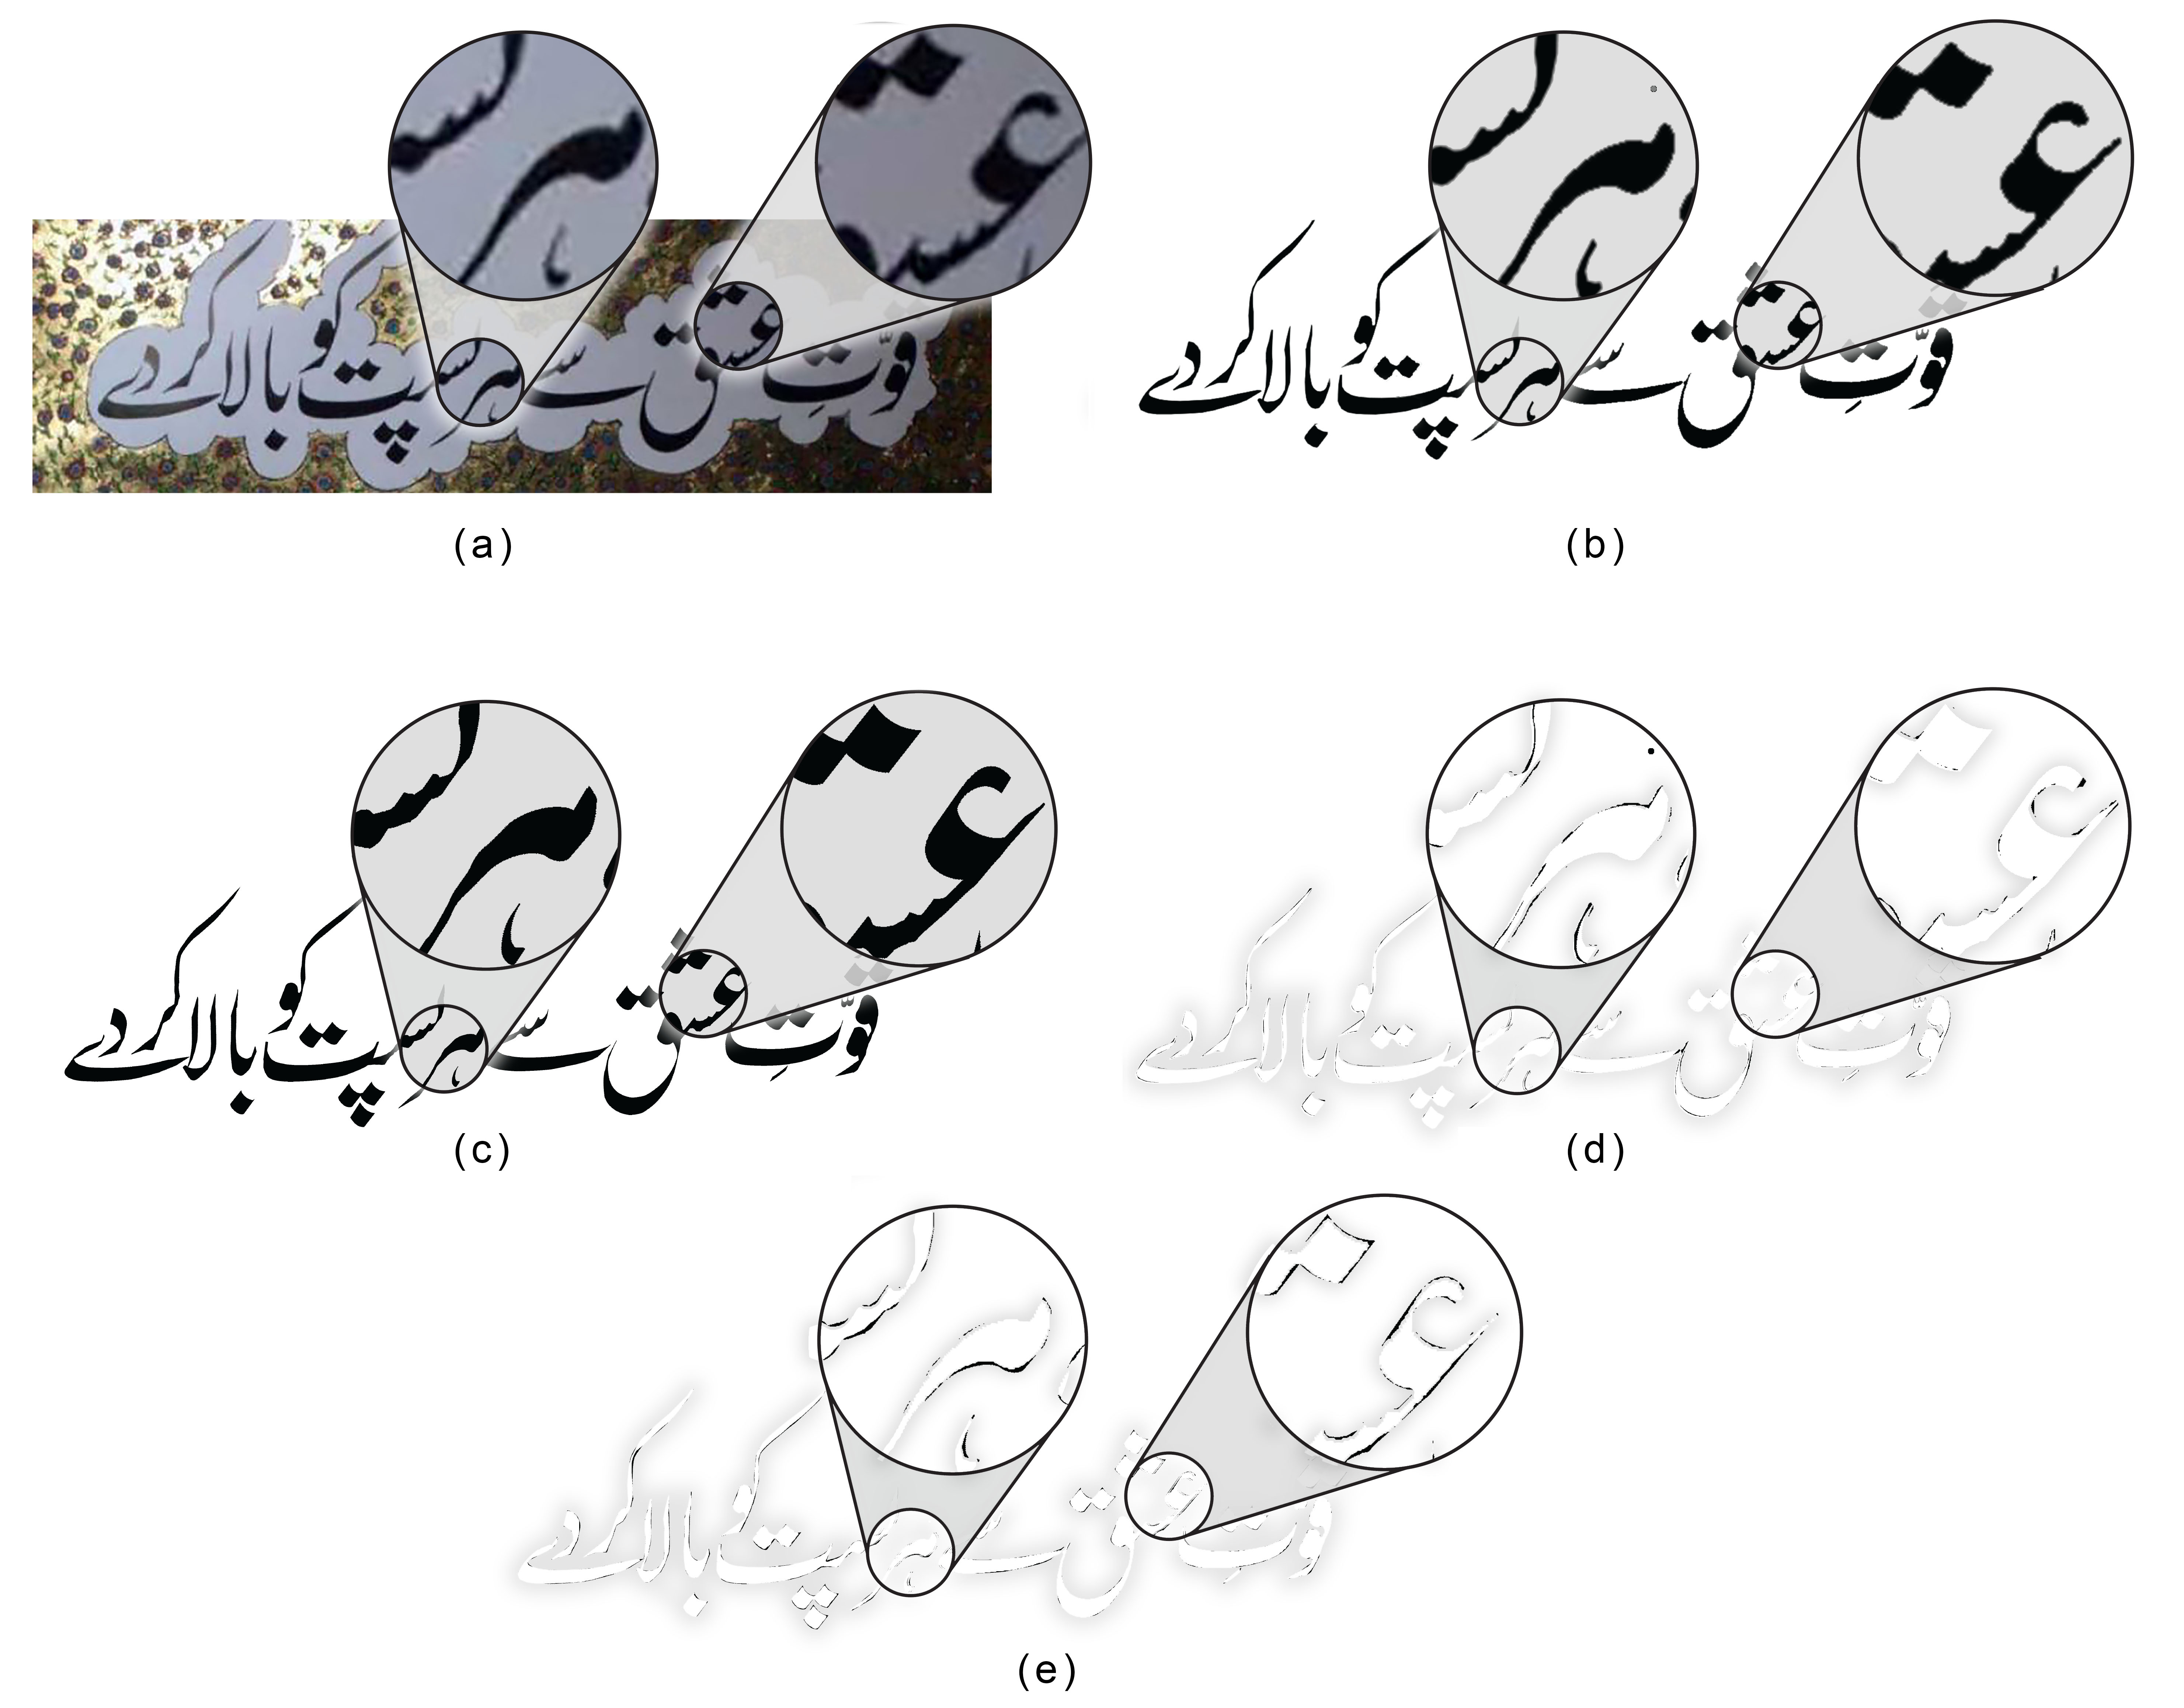
\includegraphics[width=1\textwidth]{InkComparison.jpg}
  \caption{A test comparison of the original specimen of Gohar's script and the one traced with twisting bezier splines. Each image includes magnified version of two typical areas of the script for better visibility. Also, in (d) and (e) a light shadow is added for better understanding and is not a part of the scripts. (a) Photo of the original script. (b) Inkmarks extracted using photoshop from the original image. (c) Rasterized inkmarks generated by twisting bezier spline curve. (d) Area of the original ink missing in the twisting splines. (e) Area of the ink marked outside the original ink.
  } 
  
\end{figure}
        
Figure \ref{Fig:Nastaleeq} and \ref{Fig:Thuluth} show sample outputs produced by tracing two of famous Gohar's articles in ``Nastaleeq'' and ``Thuluth'' scripts. The twisting splines do contain vector data and have no resolution but for the sake of presentation, the images have been rasterized by ``Gregor''.
\begin{figure}
  \centering
  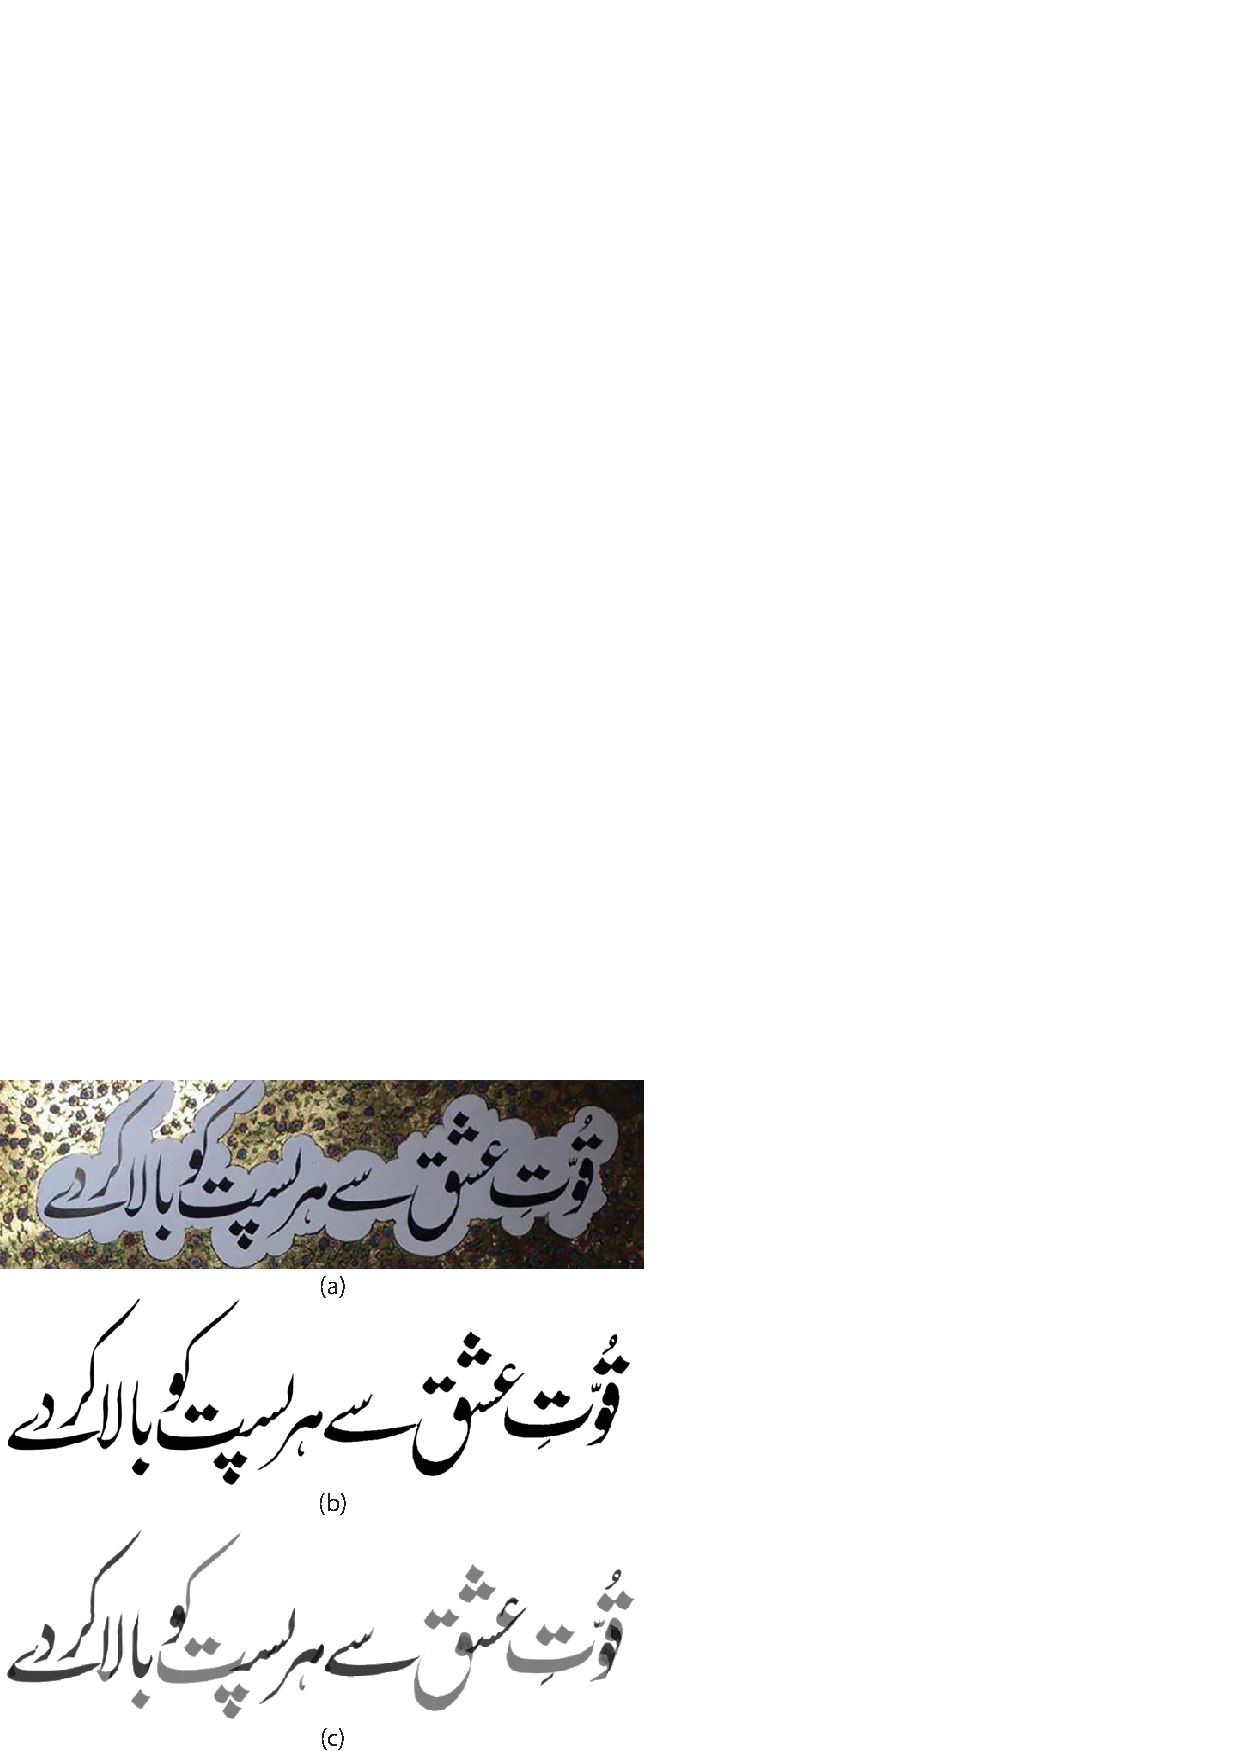
\includegraphics[width=0.6\textwidth]{NastaleeqSample.pdf}
  \caption{A specimen produced in ``Nastaleeq'' script. (a) Original photograph of the specimen (b) Rasterized binary image of the twisting spline curves. (c) Rasteriezd shaded image of the twisting spline curves highlighting individual curve parts.} 
  \label{Fig:Nastaleeq}
\end{figure}     

\begin{figure}
  \centering
  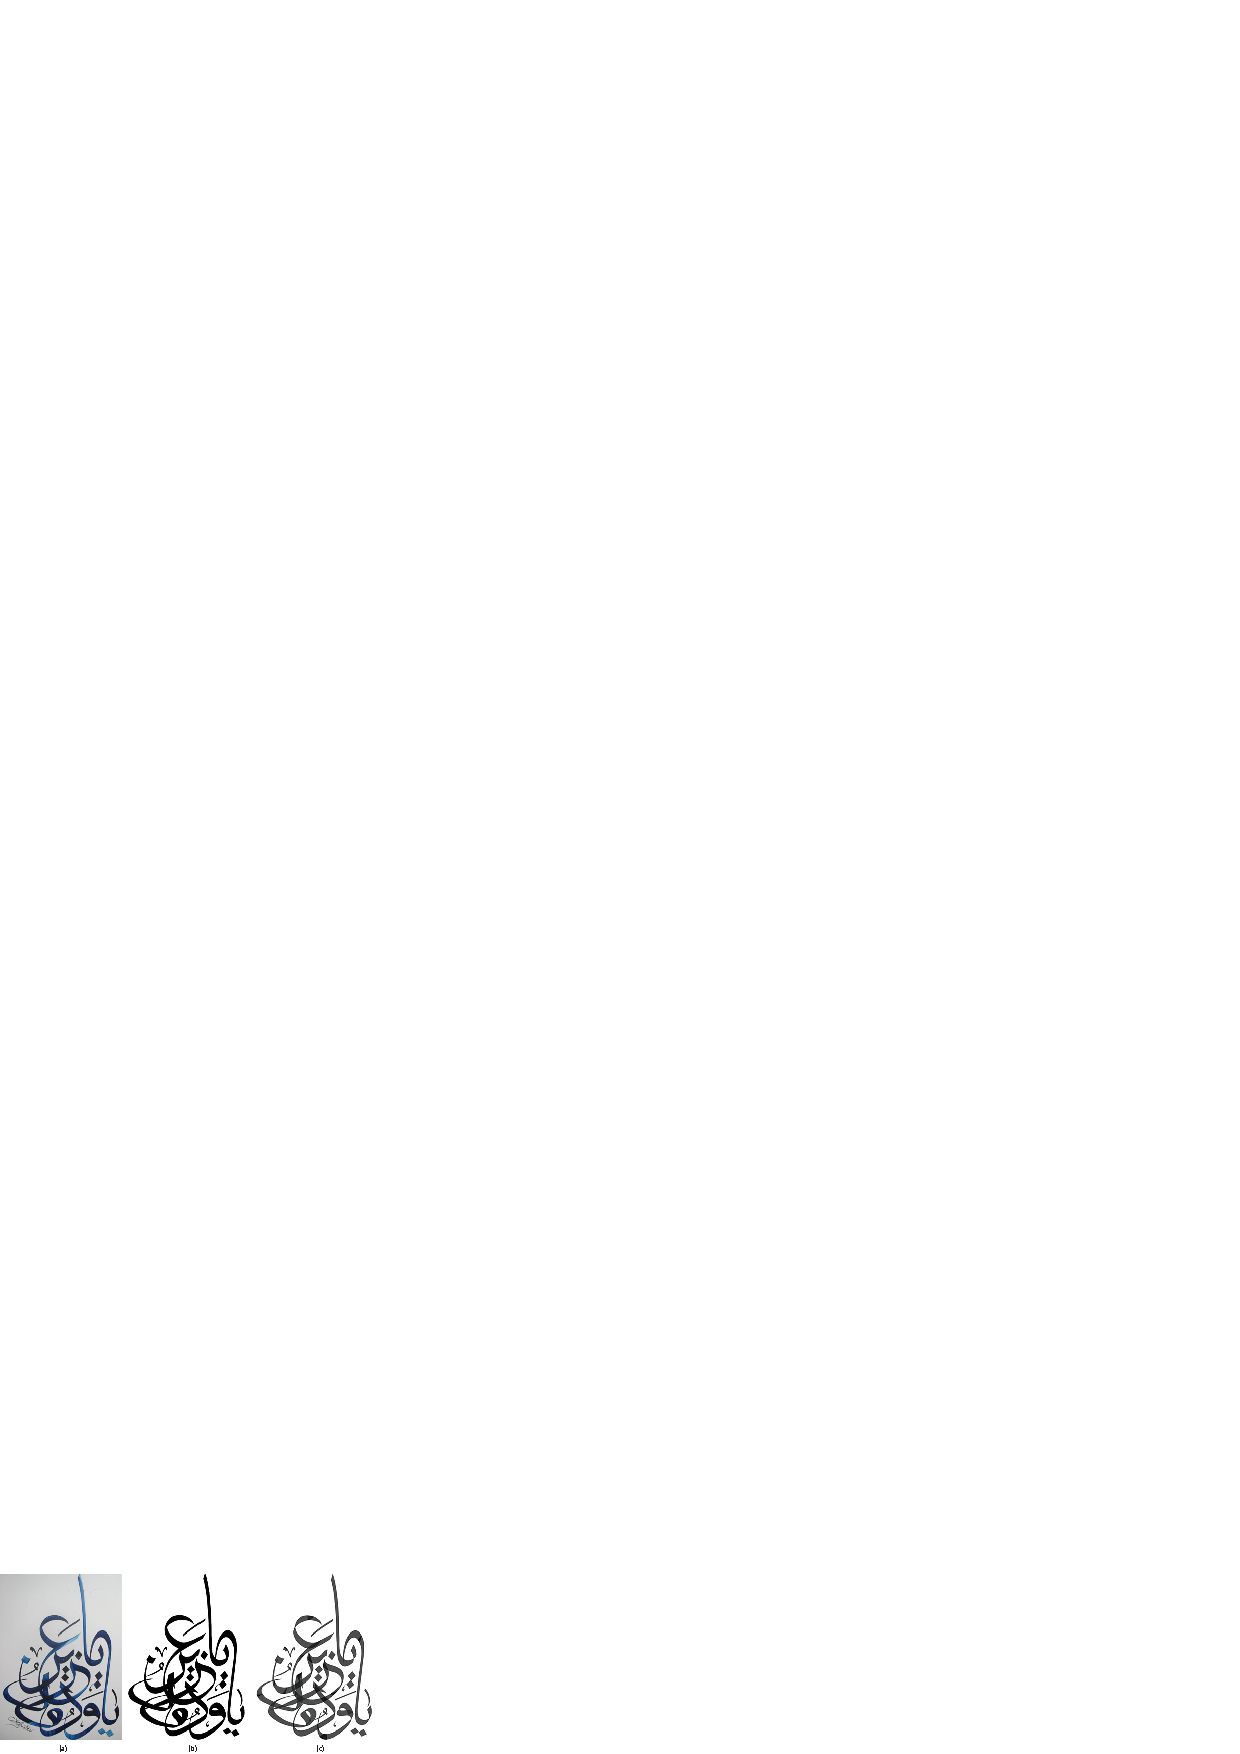
\includegraphics[width=1\textwidth]{ThuluthSample.pdf}
  \caption{A specimen produced in ``Thuluth'' script. (a) Original photograph of the specimen (b) Rasterized binary image of the twisting spline curves. (c) Rasteriezd shaded image of the twisting spline curves highlighting individual curve parts.
  }
  \label{Fig:Thuluth}
\end{figure}     

\clearpage                % Twisting Bezier Splines
\section{Robotic Manipulator}\label{chapter2}
{
    \subsection{Functional Requirements of the Manipulator}
    {
        The robot is required to perform precise maneuvers with complete $6$ degrees of freedom of the end effector in both planar and cured planes. It is also required to provide at least one extra actuator to reduce singularities. In addition to position, the robot is also required to perform precise velocity and force controlled maneuvers.
    }
    \subsection{Robot Representation}
    {
        Before going on to the selection of a robot, one unexpected issue arose when I wanted to represent my robot. Conventionally, the robot can be represented on a piece of paper using simple symbols and links as shown in Fig. \ref{FigConventionalRep}
        \begin{figure}
          \centering
          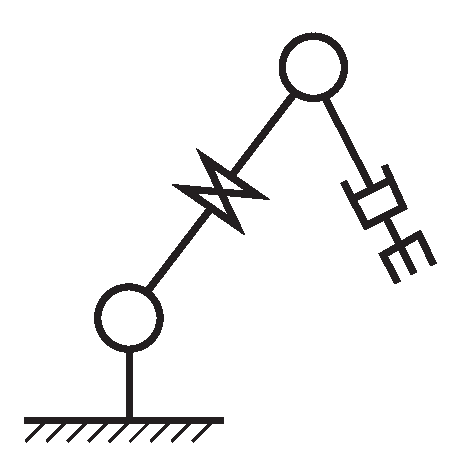
\includegraphics[width=0.5\textwidth]{RobotRep1.pdf}
          \caption{Conventional way of representing a manipulator. The circles show a rotation between the interconnected links on the plane of the paper. The cross symbol shows rotation on the link line. The square symbol is for prismatic joint. It represents change in length along the link line.}\label{FigConventionalRep}
        \end{figure}
        This kind of representation is clean and simple but doesn't give a complete view of the robot. Specially, with virtually zero link lengths, the visual representation can confuse someone new to the realm of robotic.

        Based on repeated experiments and to answer the weakness of contentional representation, let us define a new representation that encapsulates the basic idea of representation with some features of $D-H$ table. See Fig. \ref{FigMyRep}
        \begin{figure}
          \centering
          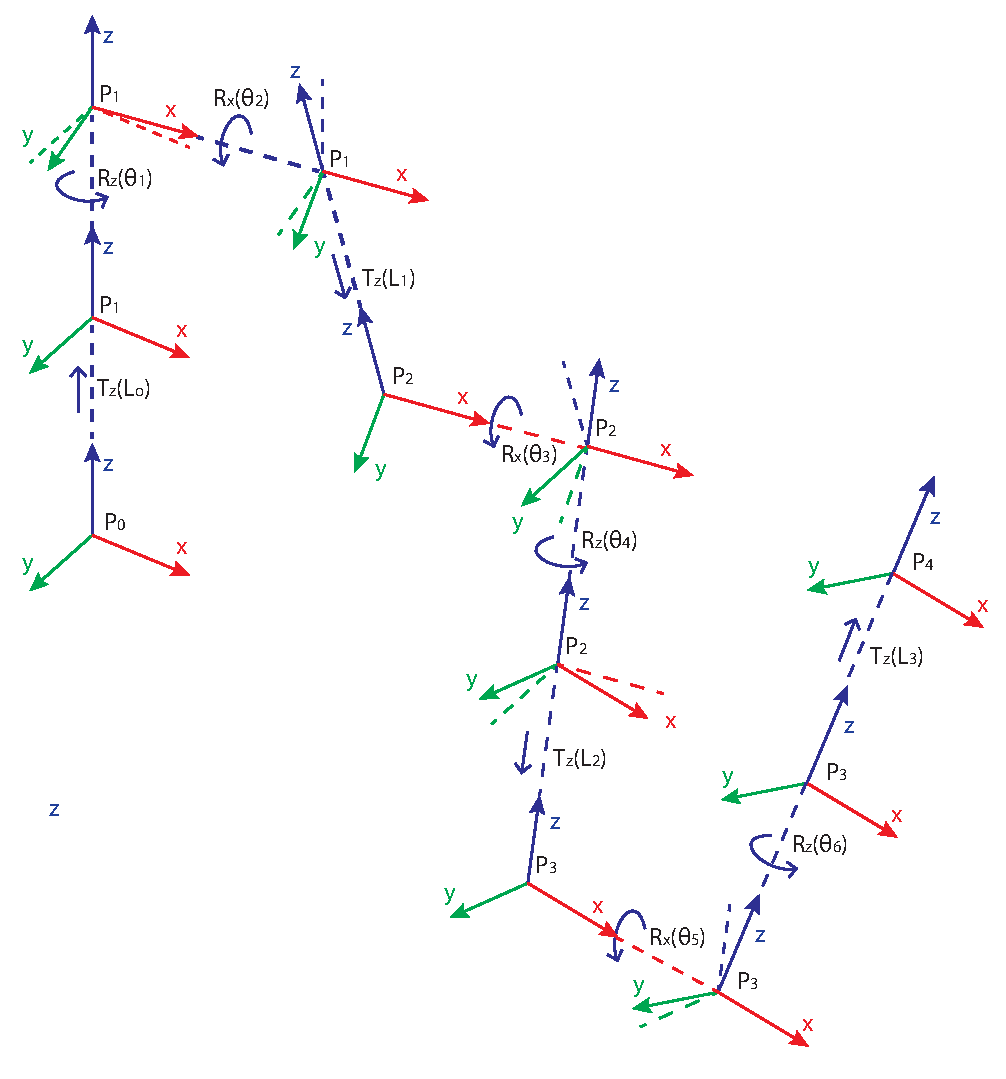
\includegraphics[width=0.8\textwidth]{MyRep.pdf}
          \caption{An example of \texttt{transformation frames} representation. This representation shows how a reference frame is linked to the previous using two basic transformation functions, $T_n$ and $R_n$ where n is the axis along or about which the transformation is performed. The schematic is drawn in the direction of $F0$ to $F_N$ ($N$ being the last frame) but can also be interpreted in reverse direction. One can easily see which transformations are required to convert one frame of reference to the other. One only needs to take one thing in account. When going in forward direction, all the transformations are applied as they are but while going back, each successive transformation is taken as inverse. For example, frame $F5$ can be achieved from frame $F3$ by applying two successive transformations: translation along $x$ of magnitude $L1$ and rotation about $x$ of magnitude $\theta_3$. However, to go to frame $F3$ from frame $F5$, one needs to apply two successive transformations: rotation about $x$ of magnitude $-\theta_3$ and translation along \texttt{x} of magnitude $-L1$. It should be noted that if a transformation changes the origin of the frame, the next frame has a different point shown at the center. This point is defined in the base frame.
          } \label{FigMyRep}
        \end{figure}

        Interestingly, this representation can't only represent physical manipulators, it can also represent abstract transformations. See Fig. \ref{FigEulerRep} which represents a target $P_t$ being represented as $z-x-z$ euler angles.

        \begin{figure}
          \centering
          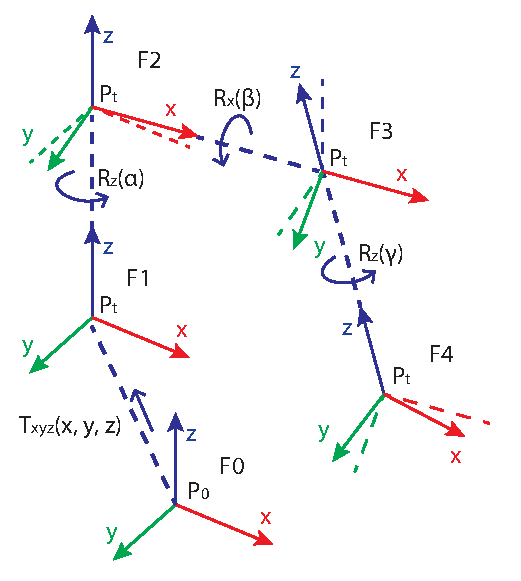
\includegraphics[width=0.6\textwidth]{EulerANgles.pdf}
          \caption{Three successive rotation $z-x-z$ and similar orders are call \texttt{Euler Angles Transformations}. A base Frame $F0$ is transformed though three translations and three euler rotations. This way, one can easily represent a target point to the robot which would have three extra components than $x$, $y$ and $z$; $\alpha$, $\beta$a and $\gamma$.
          } \label{FigEulerRep}
        \end{figure}

        Now, if one represents both target and the manipulator representation in a solved state, a closed loop representation can be formed which becomes extremely convenient in inverse kinematics. See Fig. \ref{FigCompleteRep} which exemplifies a closed loop \texttt{transformation frames} representation. It should be quite clear that once a closed loop is constructed, one can make transformations in any direction.

        \begin{figure}
          \centering
          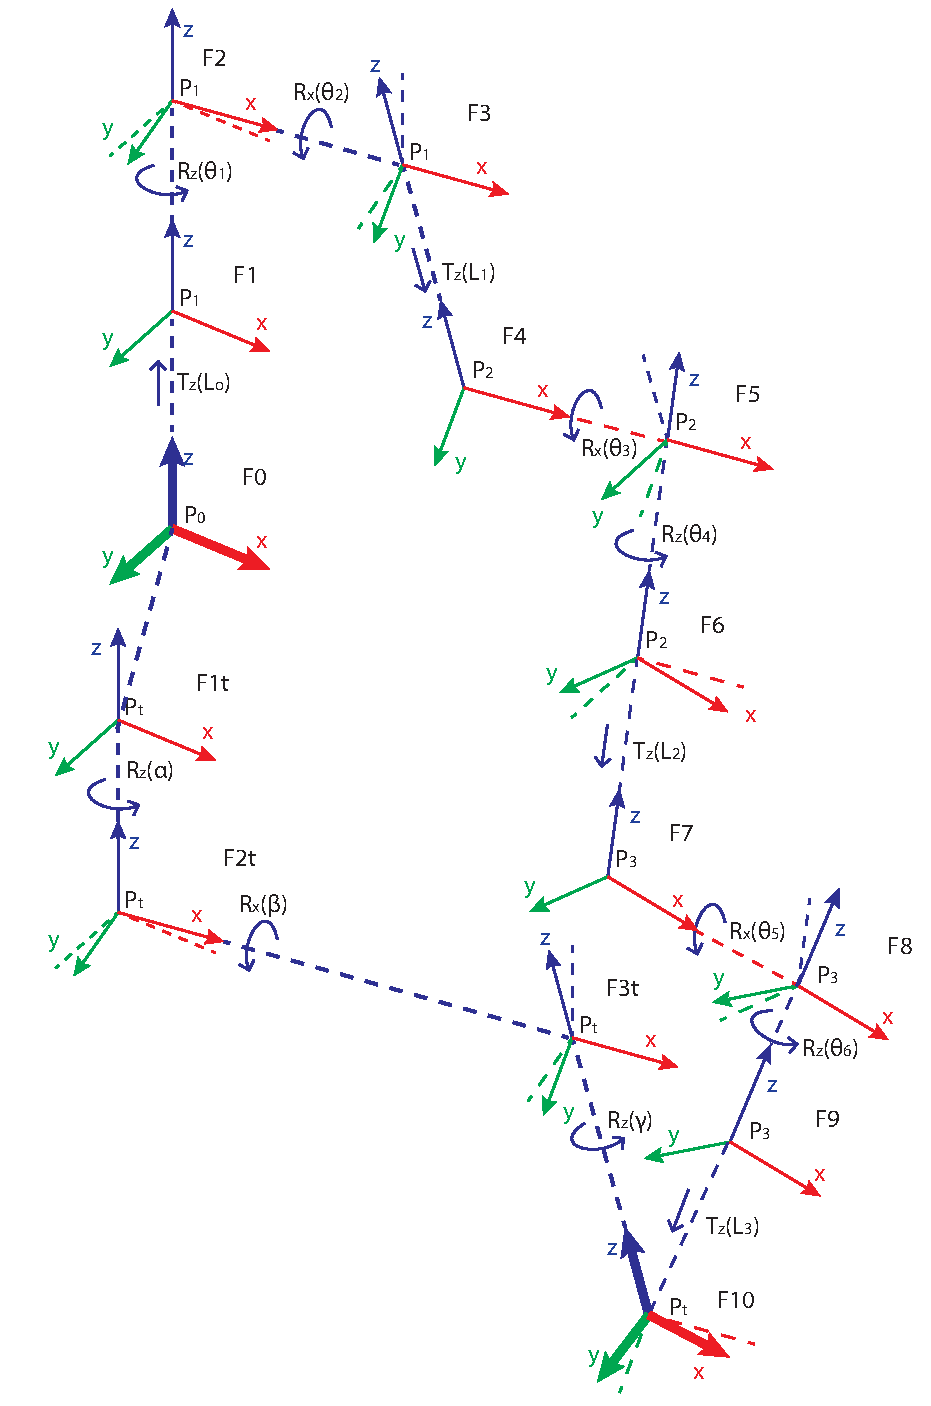
\includegraphics[width=0.9\textwidth]{CompleteRep.pdf}
          \caption{A manipulator along with a target represented in \texttt{transformation frames} representation. $F0$ corresponds to the base frame, $F0, F1, F2 ...$ represent the forward direction of the manipulator and $Ft0, Ft1, Ft2 ...$ represent the forward direction of the target. Both chains of transformations lead to a common reference frame eventually, the target frame of reference, or the end-effector frame of reference, $Ft$.
          } \label{FigCompleteRep}
        \end{figure}

        It is interesting to see that while doing a complete cycle transformation, one virtually transforms a frame through nothing! Also, if a $N-1$ frame transformation is applied in a $N$ frame closed loop, one can identify one last transformation quite easily by comparing the initial and the final frames. This method is called \texttt{Known Error Propagation} and will be used extensively in the inverse kinematics.

        Last, but not the least, of the usages of a closed loop representation is that some transformations can be skipped/swapped safely in order to simplify the loop. This can lead to finding further more unknown parameters using \texttt{Known Error Propagation}.

    }
    \subsection{Selecting a Configuration}
    {
        The configuration selected for this project is widely used by other engineers but the main inspiration behind choosing this configuration was a B.Sc. final year project of the \emph{Mechanical Engineering Department of U.E.T} of the batch $12$' with title, 'Design and Implementation of a $6$DoF Spot Welding Robot'. The project report presents a solution and describes all the forward and inverse kinematics. And all this, without using a regular transformation matrix! The effort in the current project takes some inspiration from the previous one and also elaborates not only the faults and issues with the previous but also the effectiveness of using transformation matrices.

        See Fig. \ref{FigCompleteRep} which represents this manipulator.

        In addition to these six degrees of freedom, we have attached a linear force control actuator along the end effector, since this actuator is responsible to keep the normal force under control, effectively, the robot solution remains the same as for six degrees. This scheme will be described later.
    }
    \subsection{Mathematical Modelling}
    {
        Using the new representation, properties of homogenous transformation matrices and basic highschool trigonometry,  I was able to calculate the unique and redundant solutions for the spherical manipulator. The process will be described later, but, summarily, the robot has two primary solutions: different joint positions yield the same end effector position and orientation. Connected to both solutions, are $4$ more secondary solutions which effect only the motor angles not the link locations.

        Finding out the mathematical equations is one job, verification is another. While dealing with three dimensional realm on a two dimensional paper, one can the solution but making small human errors on the way. It is quite easy to confuse the directions of rotations in a reference frames, resulting in typical errors which can be mitigated by some hit-and-trial of a few operations; adding or subtracting integral multiples of $\frac{\pi}{2}$ from the angles, inverting the length signs, inverting the angle directions. This can be done easily only if a representation tool is build alongside the robot modeling.
    }
    \subsection{Simulation and Analysis Solutions}
    {
        Even with a complete mathematical model, there are tasks which require the power of simulation either for design and planning or for the verification of the existing model. The tool used for this step is discussed in detail in the coming sections.
    }
}

    \subsection{Inverse and Forward Kinematics}
    Some of the motor angles are quite obvious. See the series of hand-sketched figures labelled with mask Fig. \texttt{RDn} in the subsequent pages which demonstrate how an inverse kinematic solution was discovered for this robot.

\subsection{The Calligraphy Job}
{
        Calligraphy is a kind of art that finds its links in the, so called, technical areas. They write and discover new fonts on the way but one thing remains the same. Whatever the idea an artist has in his mind, has finally to be represented as Ink marks which, usually, are made flat head pens and rectangular paint brushes. The tool doesn't know what actually drives it, it only knows how it should react to the specific surface and specific kind of input.

        This is where we innovate: replace the hand of the artist with a robot. The mind that imagins/creates/discovers the art, however, cannot be replaced by the robot. Or even if it can be, it would be out of scope of this project. So, now we need to create two more interfaces: between the human and the robot and second, between the robot and the writing tool.

        For the first interface, we discovered a modified form of bezier curve, "the rotation supported bezier". Bezier curves were first reported in use by a French physicist, \texttt{Paul de Casteljau} using \texttt{de Casteljau's algorithm}. He used bezier splines to model the bodies of \texttt{Renault} cars in 1959. We, after all those years, have discovered how asymmetric pen rotation can be incorporated in the bezier curves to define language scripts that require an asymmetric pen tip.

        See Fig. \ref{FigBezier} which shows a screenshot of a bezier rotation curve constructed in \texttt{Drogon v2}.

        \begin{figure}
          \centering
          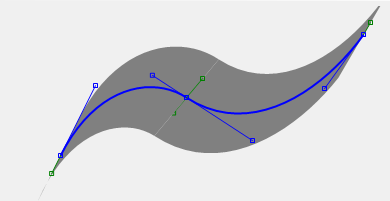
\includegraphics[width=0.7\textwidth]{bezier.png}
          \caption{A usual bezier spline has only two interlinked handles on a each anchor point which can control the shape of the curve before and after the anchor (shown blue). We have added a second (green) handle to each anchor which controls the rotation of the pen. Since the rotation handles act similar to the shapre handles, one can, in-effect, control change in rotation very accurately and smoothly.
          } \label{FigBezier}
        \end{figure}

    }
\subsection{Forward Kinematics}         % Robotic Manipulator
\section{Gregor -- The Twisting Bezier Spline Editor}\label{Chapter:Gregor}
\subsection{Introduction}
{
    The twisting Bezier splines may well mathematically be able to quite accurately contain most of the information required to replicate a calligraphy artwork but will hardly be practically useful without a tool strong enough to enable an artist to effectively trace an existing or create a new calligraphy specimen. Now, making such a tool was in itself an entire software engineering project and could not easily fit in the scope of the on going work. However with this link missing, in would have been impossible to quantitatively test and benchmark the performance of the other tools. So the least that could actually be done would be to layout the bare minimum user requirements and start writing the tool. The coding work was only as linear as any other software project which relies on ambiguous and equivocal requirements. Meaning that once the first version of the software had been built, the software had to be taken back to development many times after tests with real artists. Some features were added later to fulfil the necessity that was felt during the trial while others which were initially considered to be cardinal to working of the application.

    The name ``Gregor'' is taken from a character of George R. R. Martin's legendary novel\cite{bib19} series Game of thrones. He is one of his kind; not the fastest fighter there is but is strong and every blow of his sword is effective.

    Once the application had been developed, came another step which is often forgotten and considered dispensable usually by most developers; documenting the code and the usage. Documentation of the code and a user manual is the only thing that turns an application into a software. As said earlier, keeping in view the scope of the project, the documentation too had to be limited to contain only the most critical parts. This chapter may serve as the user manual of the software. The user guide includes:
    \begin{itemize}
      \item describing how the application should be used normally,
      \item the user interface,
      \item keyboard shortcuts,
      \item saving and loading data, and
      \item introduction to analysis tools.
    \end{itemize}
    While the coding manual includes:
    \begin{itemize}
      \item general code organization,
      \item architecture and functionality of the most important parts of the code, and
      \item the relationships between most significant entities.
    \end{itemize}
    Additionally, some snippets of the code are also included in the printed appendix and in addition to uploading the whole code as a Github repository \cite{bib20}, it can be found in appendix B which is a memory card that can be access by most computers and smart-phones.
}
\subsection{Requirements and Features}
{
    The most fundamental user requirements are very simple.
    \begin{itemize}
      \item
      {
        The most fundamental requirement was that the tool be able to let the user graphically draw a rotating bezier spline. It was not only convenient but also logical to make the editing sequence similar to other vector editing software. This will make the transfer easier for people who already have some experience in other applications.
      }
      \item
      {
        The application must be able to save and load the edited work using a data file.
      }
      \item
      {
        The user should be able to drag and zoom the view port using the mouse cursor and keyboard shortcuts.
      }
      \item
      {
        There should be a provision to load images into the workspace so that they can be traced.
      }
    \end{itemize}

    Additionally, from a developer's perspective there are some features that are either implemented inevitably along the way of implemented the essential features or the usability of these features outweighs the additional effort required for the implementation. For example, the developer would have to program at least one color that the view-port will use to visualize the splines. The effort required to just expose the color option to the user is negligible as compared to writing the rendering engine. Many such features were also made a part of Gregor.

    \begin{itemize}
    \item Toggling the visibility of curvature and rotation handles.
    \item Toggling the visibility of ink-marks.
    \item Changing the opacity and color ink-marks.
    \item Changing the viewing mode between editing and viewing.
    \item Grid snapping with an option to be toggled on or off.
    \item Changing the rendering mode of rotating bezier splines.
    \item Selecting, moving, deleting, hiding and enabling individual splines.
    \item Document explorer with thumbnails of every spline in the document.
    \item Importing splines into existing workspace
    \item Selecting, moving, deleting, hiding and enabling individual splines.
    \item Application menu to change options with keyboard shortcuts to most used menu items
    \end{itemize}
}
\subsection{Usage}
{
    The software can be used to create/trace new splines and also open up existing ones. The software uses Microsoft XML format to store data. While creating or editing a spline, the user adds more anchors by clicking on the desired position on the document. Anchors can be added to previous splines as well as the one under focus. Once a spline has been created, the user can change the thickness and color of the ink-mark and then fine tune the position of each anchor point to match the desired stroke. To trace the strokes of an existing document, the user can also load images on to the background of the document and resized and positioned at the desired position.

    Once some splines have been created, the user can choose to save the work as XML documents or be exported as images. The user can also compare the newly created artwork with the background images to analyze the false positive and false negative areas. The analysis tools can preview the difference and compute the number of pixels in each difference image.
}
\subsection{Interface}
{
    The view of the software is the spline editor with a detailed main menu as shown in Fig. \ref{Fig:GregorInterface}, document summary and a list of most commonly used toggle buttons. The application also provides some keyboard shortcuts for the most frequently used toggle options like changing the visibility of different elements and toggling the editing modes.

    The information a rotating spline contains is too much to be viewed simultaneously. The center point of the anchors, the curvature handles, twist handles, the curve, the inkmark and the background image, when displayed simultaneously is just chaotic. On top of that, when all of these elements are interactive, using a single mouse cursor to interface becomes a headache. This is why the application presents viewing and editing modes.
    \subsubsection{The Viewing Modes}
    {
        The viewing modes can be controlled using options (g1) through (g3) as shown in Fig.  \ref{Fig:GregorInterface}, the ``View'' menu (a2), or the keyboard shortcuts. There are essentially three modes of view.
        \begin{itemize}
          \item (g1) is ink and curve mode. In this mode, the splines curves and the selected handles will be shown alongwith the ink marks.
          \item (g2) is ink-only mode. In this mode, the curvature handle of the splines alongwith the anchors and the handles are hidden.
          \item (g3) is curve-only mode. The inkmark will be hidden in this mode and only the curve alongwith the selected handles will be visible.
        \end{itemize}
        it is obvious that only one mode can be activated at a moment and it can be selected either from the options (g1) through (g3) in Fig.  \ref{Fig:GregorInterface} or through the View menu. Instead of clicking on the toggle buttons, using the keyboard shortcuts can sometimes be even more convenient.
    }
    \subsubsection{The Editing Modes}
    {
        The editing models enable or disable the anchors, curvature handles and the twist handles. As shown in Fig. \ref{Fig:GregorInterface} (h1) through (h3), the editing mode toggle buttons can be used to enable or disable any of these handles. Just like the editing modes, these modes can also be controlled using the keyboard shortcuts. Unlike the viewing modes, however, these modes can be enabled all at a time. It must be noted that while in ink-only mode, none of the editing modes will have any effect of the usability of the editing handles.
    }

    \begin{figure}
      \centering
      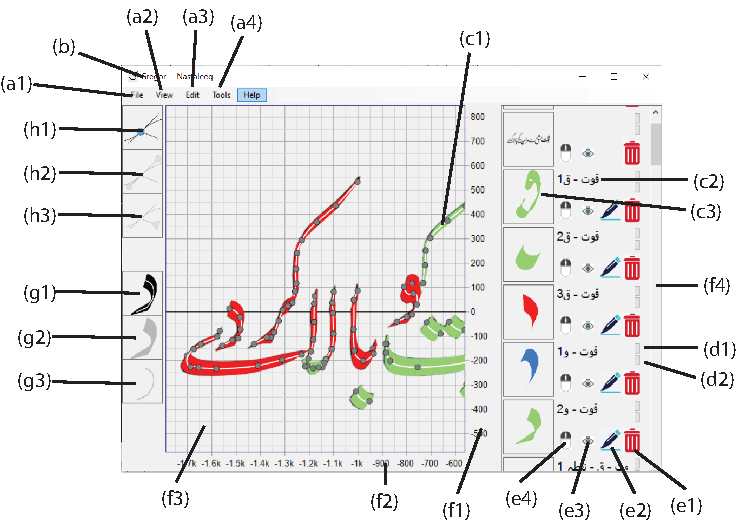
\includegraphics[width=0.9\textwidth]{GregorInterface.pdf}
      \caption{(a1-a4) The main menu options: (a1) Contains the options to open, save, import, export and clear splines and background images, (a2) enlists some viewing options; the ink viewing modes, visibility different elements of the workspace, visibility of background images, opacity of the ink-marks and rendering algorithm (a3) contains options related to editing on the workspace. It has the option to change the spline editing modes, the behaviour of left click on the workspace, and whether the splines can be dragged or not. (a4) has some analysis tools. (b) is the name of the currently open document. (c) is the main view of each spline in the document, (c2) and (c3) are the name of each spline element and its thumbnail respectively. (d1) and (d2) change the vertical order (z order) of the elements. While hovering the cursor over overlapping splines, the spline with higher position in the list will receive mouse event earlier. (e1), (e2), (e3) and (e4) are used to toggle editability, change visibility, modify color and thickness and delete the respective spline curve respectively. (f1) and (f2) are x and y axis of the workspace. (f3) is the main viewport. (f4) is the list of all the splines and images in the document. (g1) switches the view mode to both spline and inkmark, (g2) changes the viewing mode to ink only. (g3) changes the viewing mode to spline only. (h1), (h2) and (h3) toggle the visibility of center of anchor, curvature handle and the twist handle of the splines.
      } \label{Fig:GregorInterface}
    \end{figure}

}
\subsection{Modifying A Spline Curve}
{
    The application opens up an empty document by default. The first path one may choose to follow is to create new splines. This is done by adding new anchors. Anchors are added by simply clicking on an empty area of the screen. It must be noted that by default, the behaviour of the left mouse click must be switched from the Edit menu or using the keyboard shortcut to enable ``Add anchors using left mouse click''. Once an anchor has been added, adding a second anchor automatically creates a spline between the previously added anchor.
    \subsubsection{Starting a New Curve}
    {
        Since each click will append an anchor at the end of to the current spline, to break the curve and start a new one, some other procedure must be adopted. This can either be done by right clicking on an empty part of the document or toggling the ``Add anchors using left mouse click'' option off and quickly using the keyboard shortcut.
    }
    \subsubsection{Appending to a Previously Active Curve}
    {
        To append anchors at the end or the beginning of a previously active spline, simple click the center point of the first or the last center of anchor of the desired curve and it will be selected. Now, every new click will append to the selected curve just like before.
    }
    \subsubsection{Adding Anchors in the Middle}
    {
        Unfortunately adding anchor amid a curve is not a possibility yet. It would require an algorithm that can compute the nearest point on a curve from the mouse position that can show where the new anchor will be added. A work-around for now is to add anchors at the beginning or the end and soft the existing anchors inward until one of them reaches the required position.
    }
    \subsubsection{Simultaneous Curve Editing While Adding New Anchors}
    {
        It is usually very convenient to add an anchor while dragging the mouse cursor at the same time. This way, the software first adds an anchor just like it should on a mouse click but by dragging the cursor, instead of dragging the center of the newly added anchor, it drags the respective curvature handle instead. Creating new long strokes is very convenient this way. Please note that for this trick, the viewing mode must be showing the curve and both the centers and curvatures handles should be enabled.
    }
}
\subsection{Modifying an Ink-mark}
{
    \subsubsection{Adding an Ink-Mark}
    {
        Once a spline has been created with two or more anchors, the viewing mode can be switched to show ink and curve and the twist handle can be enabled while disabling the curvature handle. This will not convert the spline to a rotating curve unless it has been given a thickness. To change the thickness of a spline, simply click on it or the respective appearance in the document explorer as shown in Fig. \ref{Fig:AppearanceEditor} (e3). A curve appearance editor will pop up as shown in Fig. . Allowing to change both the broad edge thickness and the color of the ink-mark.

        \begin{figure}
          \centering
          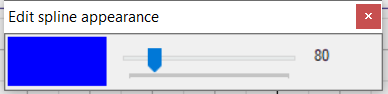
\includegraphics[width=0.3\textwidth]{appearance editor.PNG}
          \caption{The curve appearance editor lets the user modify the color and broad edge thickness of the simulated pen} \label{Fig:AppearanceEditor}
        \end{figure}
    }
    \subsubsection{Modifying the twist/rotation}
    {
        Once the Ink-mark has some thickness, it will start to show up on the viewport as well. If the rotation handles are enabled, one can start dragging each rotation handle to start twisting the curve. The artist usually continuously switches between ink and curvature handles to keep modifying the final spline until they are satisfied with the final ink-marks.
    }
}
\subsection{Using Images}
{
    Images can be imported to an existing workspace by simply selecting the menu option File > Import > Image. One can choose to import an image directly from an image file or the clipboard if the user has already copied an image using a graphics editor like a photoshop or Microsoft Paint. To view it, the background images must also be enabled from the Edit menu. Once the image is visible, the user can select a discrete handle at the middle of the image to change the placement and an anchor at the top right corner to change the size, aspect ratio, mirroring and rotation of the image.
}
\subsection{Using the Document Explorer}
{
    In addition to shoing up in the viewport, all the images and splines also appear in the document explorer as shown in Fig. \ref{Fig:GregorInterface} (f4). Each item is represented by a multi-option control which shows some controls associated with the respective item.
    \begin{itemize}
      \item Fig. \ref{Fig:GregorInterface}(c3) is a normalized thumbnail of the respective item.
      \item One can change the name of each item using Fig. \ref{Fig:GregorInterface}(c2) which can come handy while dealing with multiple items which may look similar.
      \item (e1) will delete the respective item
      \item (e2) pops up the appearance menu of the respective curve
      \item (e3) toggles the visibility of the respective item
      \item (e4) toggles the editability of an item. A Disabled item can be viewed but not interacted with.
      \item (d1) and (d2) change the order of the z-order items in a document. A simple trick while moving an item in a very long list of items is to click once on the required move button and then instead of finding the relocated button again and clicking on it again, one can now choose to press the space bar or the enter button on the keyboard which will press the button again no matter where-ever it is.
    \end{itemize}

}
\subsection{Save, Load, Export}
{
    Once the user is satisfied with the artwork, they can save it using the File menu. Once saved, the user can save any further changes to the same file by simply using the well known save command ``Control + S'' or by using the Save option from the menu again. Once saved, the file can either be opened by using the Open option in the File menu or using the windows explorer. The saved files use an extension ``rbs''. The windows usually does not recognize this extension and will thus present a list of typical applications that can open it. Choose to browse for a custom application and point to the Gregor executable. The windows will not only open the file in Gregor but also remember this choice to open rbs files in the future.

    In addition to opening a file, a user can choose to import the curves contained in a file into an existing workspace, No current items will be cleared while importing a file.

    \subsubsection{Exporting Images}
    {
        Since the curves are vector data, one may still need to export this vector into a rasterized image to be used in various circumstances. A user can export the workspace in a pixel depth of their choice using the export option in the File menu. The export window as shown in Fig. \ref{Fig:ExportMenu} presents several options
        \begin{itemize}
          \item User can control whether to include the anchors and spline curves in the render
          \item The background images can also be exported alongwith the splines.
          \item A uniform color can be selected for the exported splines.
          \item The user can also specify the rendering algorithm for the ink-mark.
          \item Last but not the least, the user can specify a pixel density. By default, each unit on the grid will be considered one pixel. Specifying a pixel density of $100$~DPU specifies to generate one hundred pixels between one unit on the grid. It must be noted that while using too dense or too large images, the application might succumb to the memory load of the procedure. So it is wise to always save the data before attempting to export an image.
        \end{itemize}

        \begin{figure}
          \centering
          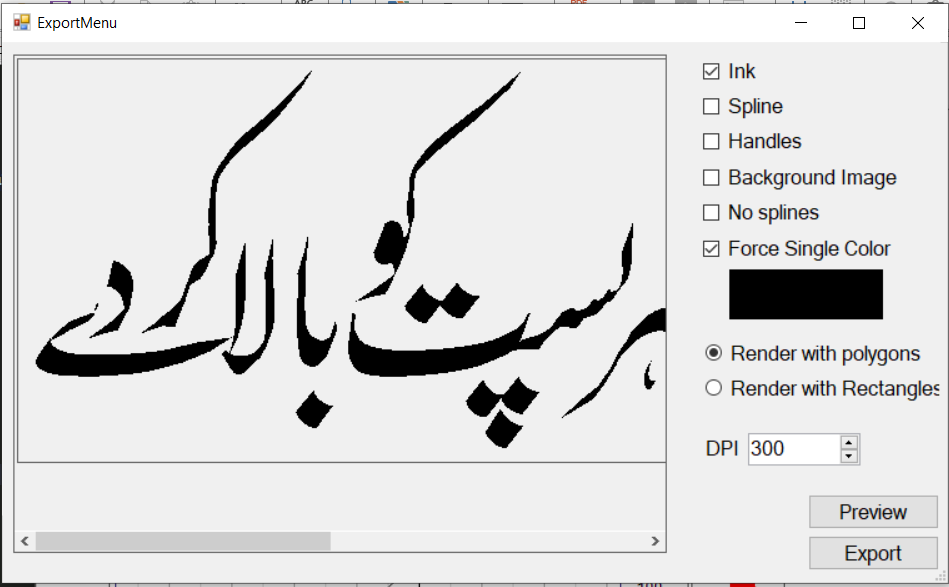
\includegraphics[width=0.9\textwidth]{ExportMenu.PNG}
          \caption{The curve appearance editor lets the user modify the color and broad edge thickness of the simulated pen} \label{Fig:ExportMenu}
        \end{figure}
    }
    \subsubsection{The File Format}
    {
        Gregor uses Microsoft XML format to save data. XML is primarily used to save text data. To pack images in it, the image is first converted into a hexadecimal list of byte data and represented as a very long string. It may inconvenience the user if they try to open it using a simple text editor which will show thousands of lines of gibberish hexadecimal bytes. One way to open the file as text is to open using an advanced raw text editor like Notepad++ or Sublime Text. These editors have the provision to collapse a certain node of an XML document, making the rest of the data more readable.
    }
}
\subsection{Short-keys}
{
    The most common keyboard shortcuts can be viewed in Table \ref{Table:Keyboardshortcuts}.
}
\subsection{Analysis Tools}
{
}
\subsection{Development}
\subsubsection{Code Organization}
\subsubsection{The BezierBoard Class}
\subsubsection{RBSPoint}
\subsubsection{Spline Elements}
\subsubsection{Miscellaneous Helper classes and form}
\subsubsection{Areas needing Improvement} 

\clearpage        % Gregor -- The Twisting Bezier Spline Editor
\section{Drogon -- The Robot Simulator}
{
    \subsection{Introduction}
     
    To effectively analyze and verify the proposed solutions, a real robot was needed. Unfortunately with the COVID-19 situation, making a real robot became almost impossible with all the supply shortages and supply chain disturbances. Simulating the manipulator becomes the second option in this case. Although its not a definitive answer but with careful assumptions, a simulator ca very well be used to verify the proposals.

    On a lighter note, just like the name Gregor, \textbf{Drogon} was also taken from a fictional character in one of the George R. R. Martin's Game of thrones novels; a mighty dragon.

    \subsubsection{The Requirements}
    Another problem was finding the best simulator to carry out the task. With no earlier training in simulators but a years of experience in programming, I decided to program an in-vitro simulator. The simulator was required to posses some important features and requirements.

    \textbf{The Simulator:}
    \begin{itemize}
      \item Simulate the position and links of the manipulator in discrete time domain.
      \item Simulate the output motors and actuators
      \item PID controllers
      \item Simulate the effect of gravity
      \item Angular and linear momentum
    \end{itemize}

    \textbf{Analysis Tools:}
    \begin{itemize}
      \item $3$~D visualizer
      \item Plotting
      \item Workspace optimizer
      \item Export data for further analysis
      \item Path planner
      \item Manual motor control
      \item Manual end effector control
      \item Machine codes parser
    \end{itemize}

    Out of all these features, there were some that could not be completed or had to be skipped given the scope of the work. Since one may be very tempted to code them or even use them, the doors to implement them are open in the code. The features are as following:
    \begin{itemize}
      \item PID controller (partly implemented)
      \item Linear and angular momentum (partly implemented)
      \item Machine code parser
    \end{itemize}

    Comprehensiveness is the core attribute of Drogon. It provides, under one screen, the flexibility to introduce an elementary change in the design, like, the maximum speed of an actuator and directly observe the consequences on all of the analysis tools. One can choose to programmatically or manually signal an actuator to move in a particular direction and position, and visualize the outcome in a $3$D preview window. It also integrates with Gregor to support the live editing and visualization of rotating bezier spline curves

    Besides comprehensiveness, our design tool offers a set of powerful analysis tools which enabled us to solve complex robot maneuvers and optimize the solution. Performing mechanical simulation with simplified real world constraints, $3$D live preview of the moving robot, work-space optimizer, $2$D art drawing, investigating the actuator velocity in continuous and discrete demain are some of the tools we used for optimization in our design.

    Since the tool is based on in-vitro coding, it can be taught to easily integrate with and inside Microcontrollers to practically , Proteus and SolidEdge to give more design flexibility.

    \subsection{The working principal}
    In this section we discuss the working principals of different aspects of the simulator.

    \subsubsection{Simulation}
    The simulator used in this work is designed from scratch. It is highly customizable in terms of coding and usage. In one configuration it can simulate a manipulator based on steppers motors. This way, the complexity of implementing the effect of gravitational and reactional forces on each actuator. In another configuration, it can simulate actuators with a limited output power, torque/force, response time and even a feedback mechanism making them essentially servo actuators. Not all of the actuators have to this way and the governing limits can also be changed at run-time. Just like the first one, in this configuration too, it first uses forward kinematics of the robot to find out the required position of its actuators to achieve a particular end-effector position and orientation. Unlike stepper motors that can just take a required number of steps in a limited time to achieve a certain position regardless of the load it has to carry, for a servo actuator, the simulator has to calculate the gravitational loads on individual links and propagate the forces and torques to individual actuator. The controller of the actuator is, in parallel, deciding how much output it must produce. Once the simulator has both the forces on each joint, it can calculate the accelerations. And once the accelerations are calculated, it only needs to be integrated with each \emph{tick} of the simulator to yield velocity and position of the actuator. At this point, it may become quite clear that implementing the gyroscopic effects of the links become quite a challenge. Since the robot being analyzed is not supposed to be working at high speeds and loads, the error caused by ignoring this effect in approximation would be negligible.

    \subsubsection{Motor controller}
    One can choose to use either a stepper motor or a DC servo on every joint. In case of stepper motors, one can configure:
    \begin{itemize}
      \item number of steps per revolution, and
      \item minimum step time.
    \end{itemize}
    In this case the simulator assumes:
    \begin{itemize}
      \item the step time remains the same regardless of the motor speed, and
      \item the motor can take a step regardless of the applied load.
    \end{itemize}
    While in case of a servo motor one can configure:
    \begin{itemize}
      \item the maximum input electrical power,
      \item the maximum torque,
      \item maximum idle acceleration,
      \item maximum velocity, and
      \item the \emph{P}, \emph{I} and \emph{D} parameters of the controller.
    \end{itemize}
    In this case, the simulator assumes that:
    \begin{itemize}
      \item the motor are $100$~% energy efficient,
      \item they are weightless, as in they are installed in the base of the robot with mechanical links transferring the power through the arm,
      \item at a constant power, the torque reduces inversely with speed ($Power = torque \times speed$), and
      \item the PID controllers operate independently.
    \end{itemize}

    Moreover, the PID controllers work on a very simple equation
    Later on, it was discovered that implementing simple PID controllers that take the required position as reference were not very effective. So the actuators are kept as stepper motors by default and can be changed to servo motors. Work is still needed to either fine tune the PID controllers or even run them on a more powerful controller.

    More details on the working principles of the simulator will be discussed in later chapters. Also, the installation and usage of the tool is described in detail in Appendix B.

    \subsubsection{Workspace}
    The workspace contains a spherical manipulator as discussed in chapter \ref{chapter2}. The simulator considers the robot fixed on a horizontal surface at the origin $(0, 0, 0)$ with the first link along the vertical axis.

    \subsection{About the Tools}

    An shape independent model of the robot under simulation can be visualized in real time using ``$3D$ Animation'' tool as seen in Fig. \ref{Fig3D}. The ``Robot Feet Position'' tool gives a superior insight on the stability of the robot. It can be seen in Fig. 1A(e) that the center of gravity plot can help optimize the motion where stability is a concern. Using the trajectory of the center of the robot in the global frame of reference can help determine the most efficient actuator movements which can be used to displace the robot from a specific position. Screen shots of the plot produced using the ``Top Trajectory'' tool can be seen in Fig. 1A(d).


        \begin{figure}
          \centering
          \includegraphics[width=0.7\textwidth]{3D.png}
          \caption{A screenshot of the $3$D representation tool. The blue sphere under the end effector shows the target given to the robot.
          } \label{Fig3D}
        \end{figure}

    All of the tools can output in real time. The robot configuration and other parameters change with time, producing animations which make it easier to decipher the underlying information.

    \subsection{Workspace Optimization}
    The workspace optimizer allows to simulate the robot solution recursively through discrete sections of the defined workspace and evaluates the degrees of freedom the robot has  specific parts of the workspace. It then colors the segments to give a more clear idea of the robot workspace. The user can then modify the robot and see, in-result, the change in the workspace. A typical output of the workspace is show in Fig.

        \begin{figure}
          \centering
          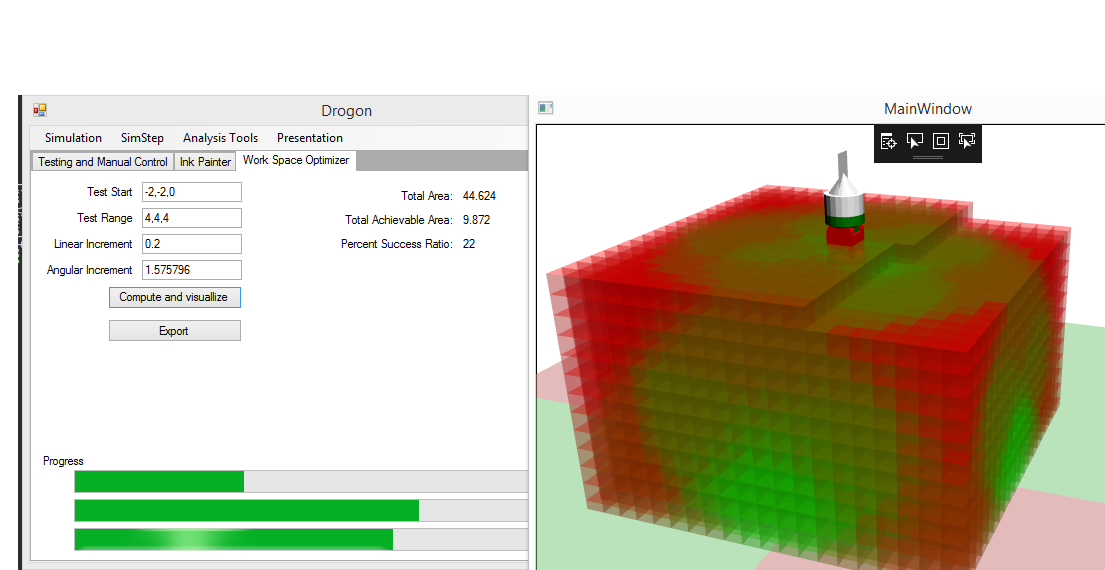
\includegraphics[width=0.9\textwidth]{WorkSpaceOptimer.png}
          \caption{The workspace is coded in colors. Purely green blocks represent a point where the robot has all of the degrees of freedom and the slightly red blocks indicate the parts where robot starts to loose one or more degrees of freedom.
          } \label{FigWorkspace}
        \end{figure}
    \subsection{Script Path Planner}
    As already mentioned, I've included a tool to construct bezier rotation splines in the tool which can serialize the data in computer files and also load from existing files. A screenshot can be seen in Fig.

        \begin{figure}
          \centering
          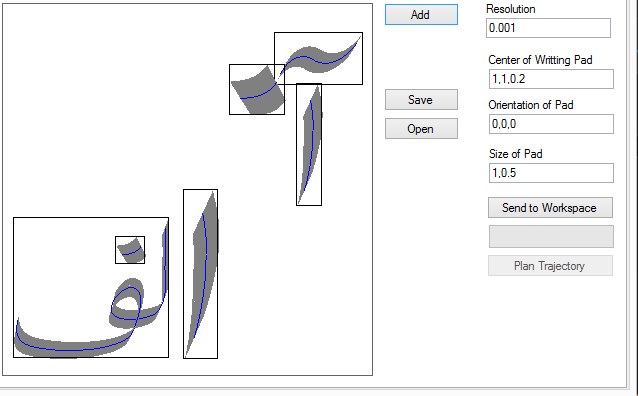
\includegraphics[width=0.9\textwidth]{SctiptEditor.png}
          \caption{The script maker can manage multiple splines and render robot trajectory according to the user resolution requirement.
          } \label{FigWorkspace}
        \end{figure}
    \subsection{Script Motion Simulator}
    Once the script is constructed using the script maker, it can be transported to the workspace in any orientation. The robot then plans how to make the required maneuvers and sibilates the behaviour. A screenshot of a robot writting a script can be seen in figure \ref{FigScriptMotion}
        \begin{figure}
          \centering
          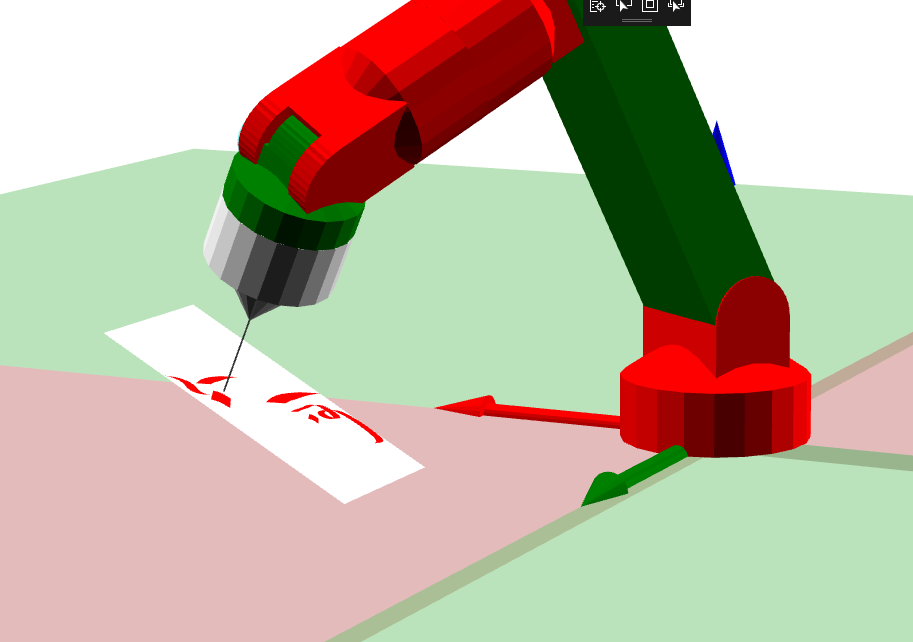
\includegraphics[width=0.9\textwidth]{writting.PNG}
          \caption{Robot writting on a slanted plane.
          } \label{FigScriptMotion}
        \end{figure}
}
\subsection{Requirements and Features}
\subsection{3D Visualizer}
\subsection{Workspace Optimizer}
\subsection{PID Tuner}
\subsection{Rotating Spline Importer}
\subsection{Usage}
\subsection{Interface}
\subsubsection{Manual Control}
\subsubsection{Analysis Tools}
\subsection{Development}
\subsubsection{Code Organization}
\subsubsection{The SphericalRobot Class}
\subsection{Simulation}
\subsubsection{Assumptions and Limitations}
\subsubsection{Accuracy of simulated Quantities}
\subsubsection{Forward Kinematics}
\subsubsection{Rotating Bezier Spline Curves}
\subsection{Sample Results}
\subsubsection{Accuracy}
\subsection{Areas that Need Improvement}
        % Drogon -- The Robotic Simulator
%\section{The Project}
\subsection{Set Milestones}
\subsection{Expected Outcomes}
\subsection{Missed milestones}

\clearpage        % The Project
\section{Conclusion} \label{Chapter:Conclusion}
{
    The twisting Bezier spline curves very closely mimic the ink mark of broad edge tools. An artist can not only trace existing calligraphy scripts, but also create an modify new ones with a very lean learning curve. The ease of use assures that the focus of the artist is more on the art itself than the caveats of the software solution. Once a script is ready, it can be imported in the robotic simulator to be tested on a real robot. Since the position and speed information about the end effector is all there, with a very little effort, one can create a translator that can convert this data into a flavor that the machine prefers; like G-Codes. The simulator is written in a fashion that with some effort it possible to create a communication bridge that lets it communicate with a real instance of a similar robot. This way, the simulator can be turned into a controller as well and that for a real small scale robots.
}
\clearpage
\begin{thebibliography}{99}
\bibitem{bib01} Web page of Baytulhabeeb, an artist, \url{https://bit.ly/islamic_cal_history}, accessed on Sep 4, 2020.
\bibitem{bib02} Arabetics™, a private foundry and consulting firm, specializing in Arabic type and lettering designs, “Roots of Modern Arabic Script:  From Musnad to Jazm”, \url{https://bit.ly/islamic_cal_history_2}, accessed on Sep 4, 2020.
\bibitem{bib03} “Islamic Calligraphy”, \url{https://bit.ly/Islamic_cal_wiki}, accessed on Sep 4, 2020.
\bibitem{bib04} By Julia Kaestle , “Arabic calligraphy as a typographic exercise”, \url{https://bit.ly/cal_styles}, accessed on Sep 4, 2020.
\bibitem{bib05} Haji Noor Den, Portfolio, \url{http://www.hajinoordeen.com/about.html}, accessed on Sep 4, 2020.
\bibitem{bib06} Mohammad Zakrya, Portfolio, \url{https://mohamedzakariya.com}, accessed on Sep 4, 2020.
\bibitem{bib07} Kamel Al Baba, Mokhtar Al Baba, Portfolio, \url{http://www.arabiccalligraphy.com}, accessed on Sep 4, 2020.
\bibitem{bib08} Abed Yaman, “A look at the history of Arabic calligraphy” \url{https://bit.ly/islamic_cal_stages}, accessed on Sep 4, 2020.
\bibitem{bib09} M. A.-de Lemos, and E. V. Liberado, “Industrial robotics applied to education”, Proceedings of 2011 International Conference on Computer Science and Network Technology.
\bibitem{bib10} Robotics in Agriculture: Types and Applications, \url{https://bit.ly/ind_robots_in_agri}, accessed on Sep 4, 2020.
\bibitem{bib11} A robot playing table tennis, \url{https://www.kuka.com/timo}, accessed on Sep 4, 2020.
\bibitem{bib12} A printing robot, \url{https://bit.ly/ind_robot_cal}, accessed on Sep 4, 2020.
\bibitem{bib13} M. Bilal, A. Raza, M. Rizwan, M. Ahsan, H. F. Maqbool, S. Abbas Zilqurnain Naqvi, “Towards Rehabilitation of Mughal Era Historical Places using 7 DOF Robotic Manipulator”, in Proceedings, IEEE International Conference on Robotics and Automation in Industry, pp. 1-6, 2019.
\bibitem{bib14} GIMP, GNU Image Manipulation Program Developers Resources, \url{https://bit.ly/gimp_developers}, accessed on July 7, 2021.
\bibitem{bib15} Inkscape Extensions, \url{https://bit.ly/inkscape_developers}, accessed on July 7, 2021.
\bibitem{bib16} Wacom Intuos, \url{https://bit.ly/wacom_intuos_official}, accessed on July 7, 2021.
\bibitem{bib17} Lenovo Thinkpad x380, \url{https://bit.ly/lenovo_thinkpad_x380}, accessed on July 7, 2021.
\bibitem{bib18} Microsoft Surface Pro 7, \url{https://bit.ly/ms_surface_pro_7}|, accessed on July 7, 2021.
\bibitem{bib19} George R. R. Martin, \emph{``A Game of Thrones''}, Chapter $30$.
\bibitem{bib20} Project code repository on GitHub, \url{https://github.com/umartechboy/Thesis_2017-MS-MC-17}|, accessed on August 8, 2021.
    \end{thebibliography} 
\appendix
\section{Tables}
\subsubsection{Gregor -- Keyboard Shorcuts}
{
    \begin{tabular}{|c|l|}
      \hline
      % after \\: \hline or \cline{col1-col2} \cline{col3-col4} ...
      Key & Action \\
      \hline
      \multicolumn{2}{|c|}{The File Menu} \\
      \hline
      Ctrl + O & Open an existing document \\
      Ctrl + S & Save the document to the last selected file or a new file if no previous file is associated. \\
      Ctrl + Shift + S & Save the data in a new file \\
      Ctrl + I & Import spline data from file \\
      Ctrl + E & Open up the export menu \\
      Shift + Del  & Clear the workspace \\
      Alt + F4 & Close the application \\
      \hline
      \multicolumn{2}{|c|}{The View Menu} \\
      \hline
      Ctrl + 4 & Combined Mode; Shows both ink and curves \\
      Ctrl + 5 & Ink Only Mode; Shows Only the ink marks and hides the curve alogwith the handles \\
      Ctrl + 6 & Splines Mode. Hides the ink marks \\
      Ctrl + G & Toggle the visibility of the grid \\
      Ctrl + Shift B & Toggle the visibility of the background images \\
      \hline
      \multicolumn{2}{|c|}{The Edit Menu} \\
      \hline
      Ctrl + 1 & Toggles the splines anchor centers \\
      Ctrl + 2 & Toggles the splines curvature handles \\
      Ctrl + 3 & Toggles the rotation handles \\
      Ctrl + V & Toggles the action of mouse left click between adding the anchor and dragging the workspace. \\
      \hline
      \multicolumn{2}{|c|}{Help}\\
      \hline
      F1 & Shows quick help \\
      F2 & Opens up the project Git.\\
      \hline
    \end{tabular}\label{Table:Keyboardshortcuts}
}
\clearpage
\section{Source Code}\label{Appendix:sourceCode}
{
\clearpage }
\section{Videos}\label{Appendix:sourceCode}
{
\clearpage }
\section{Code Snippetes}
{
\begin{lstlisting}[language=XML]
//Sample code of a rotating Bezier spline that will render the Urdu letter Aa'en in Nastaleeq.
<spline>
    <FlatTipWidth>150</FlatTipWidth>
    <Color>-5658199</Color>
    <anchor>
      <rotationoffset>0</rotationoffset>
      <P>-198.3791, 452.6993</P>
      <C1>-131.6351, 572.4461</C1>
      <C2>-265.1234, 332.9534</C2>
      <R1>-148.3791, 452.6993</R1>
    </anchor>
    <anchor>
      <rotationoffset>0</rotationoffset>
      <P>-296.5323, 156.2775</P>
      <C1>-439.8357, 254.4304</C1>
      <C2>-119.5302, 35.04326</C2>
      <R1>-246.5322, 156.2775</R1>
    </anchor>
    <anchor>
      <rotationoffset>0</rotationoffset>
      <P>25.40986, 374.1774</P>
      <C1>-47.22344, 262.2825</C1>
      <C2>98.04301, 486.0714</C2>
      <R1>75.40986, 374.1774</R1>
    </anchor>
    <anchor>
      <rotationoffset>0</rotationoffset>
      <P>-233.7143, -183.332</P>
      <C1>-208.1945, -28.25013</C1>
      <C2>-274.7982, -432.9961</C2>
      <R1>-183.7143, -183.332</R1>
    </anchor>
    <anchor>
      <rotationoffset>0</rotationoffset>
      <P>315.9428, -517.0526</P>
      <C1>95.77186, -679.5702</C1>
      <C2>435.6645, -428.6809</C2>
      <R1>365.9427, -517.0526</R1>
    </anchor>
    <anchor>
      <rotationoffset>0</rotationoffset>
      <P>441.5787, -144.0708</P>
      <C1>388.576, -277.5591</C1>
      <C2>494.5813, -10.58265</C2>
      <R1>491.5787, -144.0708</R1>
    </anchor>
  </spline>
\end{lstlisting}
}
\section{Images}
{   

\begin{figure}[H]
  \centering
  \includegraphics[width=0.8\textwidth]{Nastaleeq_Ink.pdf}
  \caption
  {
      Nastaleeq sample by Gohar Qalam. (a) Original calligraphy photo. (b) Original photo processed for analysis. (c) Traced rotating bezier spline ink. (d) Difference between (b) and (c). The red pixel indicate the portions that are missing in (c) but are present in (b) and the blue ones show the missing pixels in (b) but are present in (c).
  }
\end{figure}

\begin{figure}[H]
  \centering
  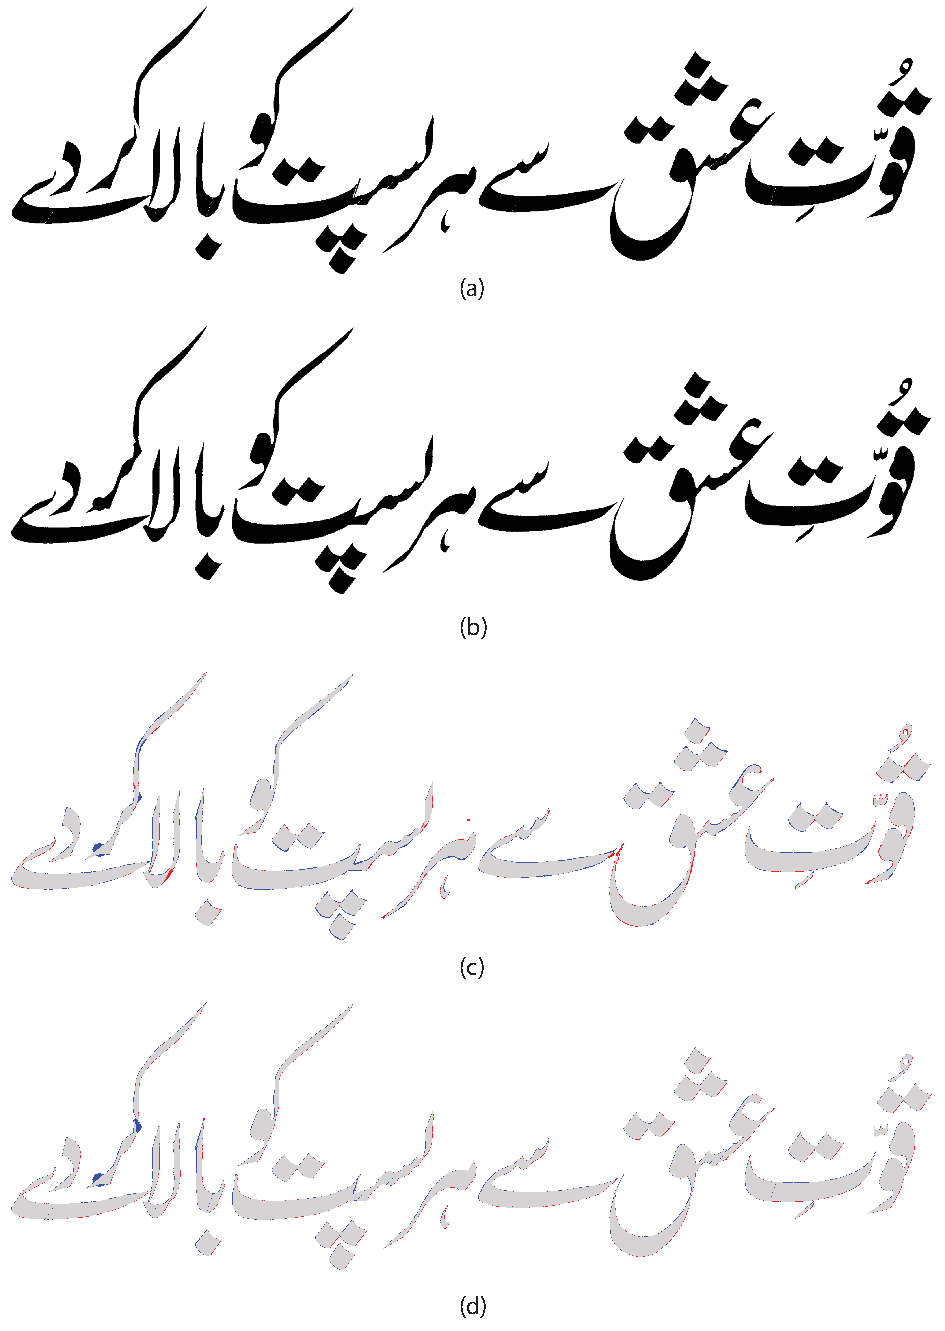
\includegraphics[width=0.8\textwidth]{Nastaleeq_Machined.pdf}
  \caption
  {
      Machined Nastaleeq sample by Gohar Qalam. (a) Rasterized rotating bezier spline for machining (b) Ink marks machined by a simulated robotic manipulator. (c) and (d) are differences between simulated ink mark and the rasterized photo and the processed original photo respectively. The red pixel indicate the portions that are missing in (c) but are present in the reference image and the blue ones show the missing pixels in reference but are present in the ink mark.
  }
\end{figure}

\begin{figure}[H]
  \centering
  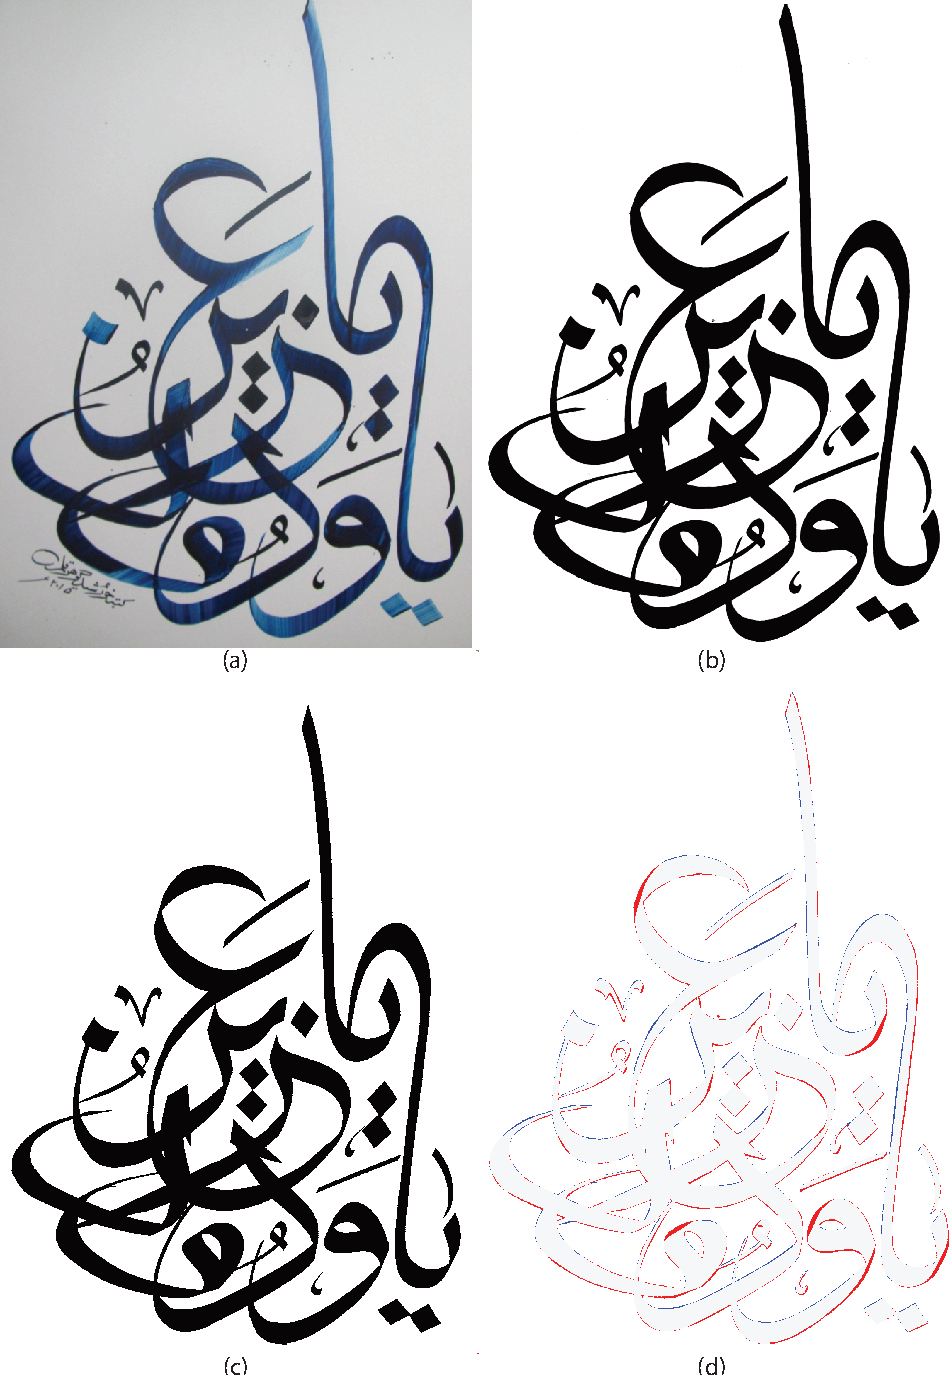
\includegraphics[width=0.8\textwidth]{Thuluth_Ink.pdf}
  \caption
  {
      Thuluth sample by Gohar Qalam. (a) Original calligraphy photo. (b) Original photo processed for analysis. (c) Traced rotating bezier spline ink. (d) Difference between (b) and (c). The red pixel indicate the portions that are missing in (c) but are present in (b) and the blue ones show the missing pixels in (b) but are present in (c).
  }
\end{figure}

\begin{figure}[H]
  \centering
  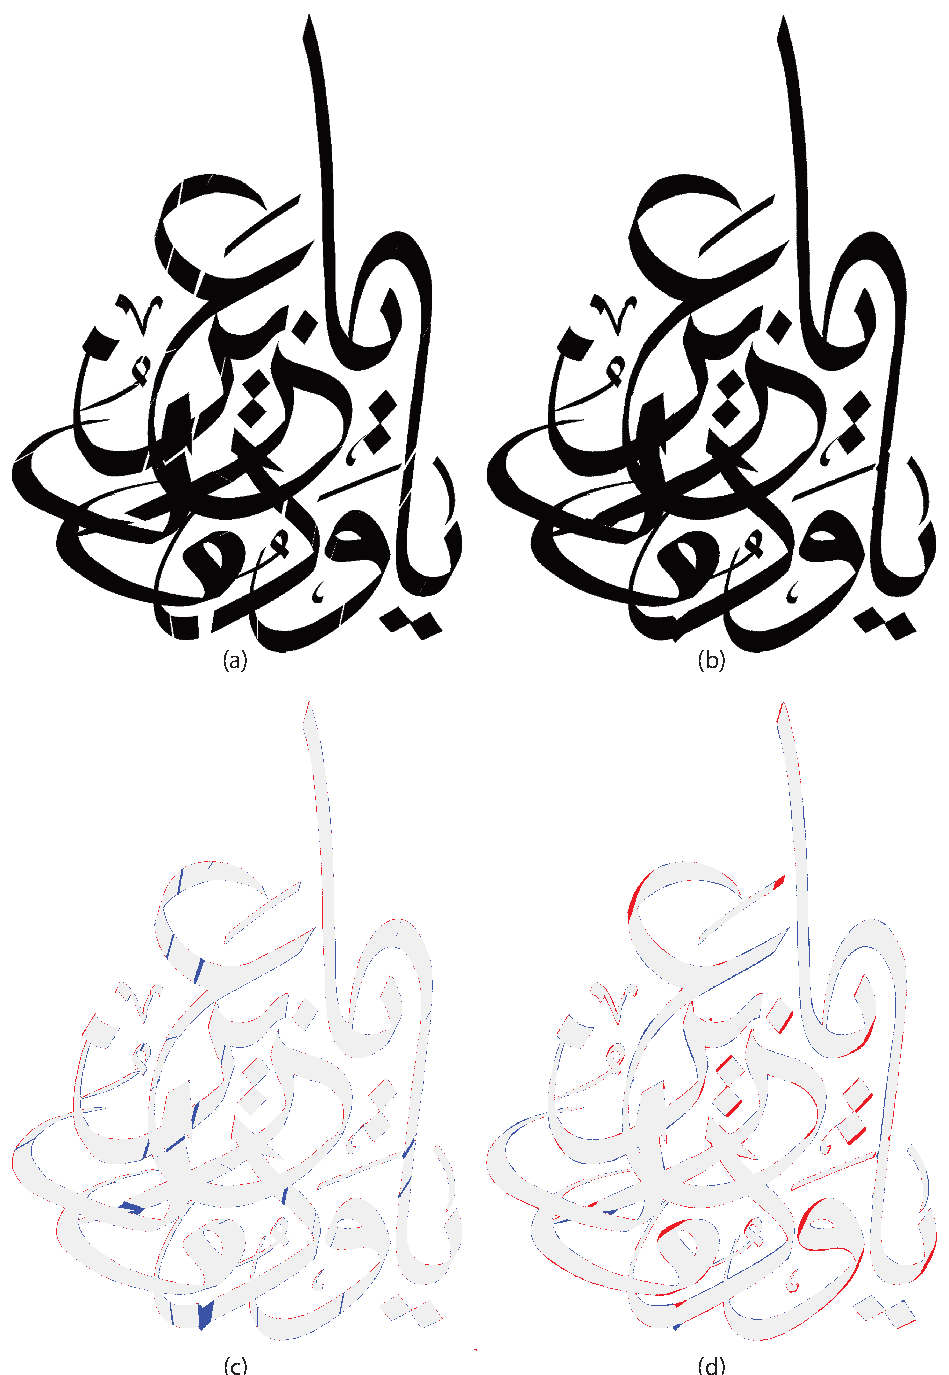
\includegraphics[width=0.8\textwidth]{Thuluth_Machined.pdf}
  \caption
  {
      Machined Thuluth sample by Gohar Qalam. (a) Rasterized rotating bezier spline for machining (b) Ink marks machined by a simulated robotic manipulator. (c) and (d) are differences between simulated ink mark and the rasterized photo and the processed original photo respectively. The red pixel indicate the portions that are missing in (c) but are present in the reference image and the blue ones show the missing pixels in reference but are present in the ink mark.
  }
\end{figure}
}
\section{Gregor -- The Twisting Bezier Spline Editor}\label{Chapter:Gregor}
\subsection{Introduction}
{
    The twisting Bezier splines may well mathematically be able to quite accurately contain most of the information required to replicate a calligraphy artwork but will hardly be practically useful without a tool strong enough to enable an artist to effectively trace an existing or create a new calligraphy specimen. Now, making such a tool was in itself an entire software engineering project and could not easily fit in the scope of the on going work. However with this link missing, in would have been impossible to quantitatively test and benchmark the performance of the other tools. So the least that could actually be done would be to layout the bare minimum user requirements and start writing the tool. The coding work was only as linear as any other software project which relies on ambiguous and equivocal requirements. Meaning that once the first version of the software had been built, the software had to be taken back to development many times after tests with real artists. Some features were added later to fulfil the necessity that was felt during the trial while others which were initially considered to be cardinal to working of the application.

    The name ``Gregor'' is taken from a character of George R. R. Martin's legendary novel\cite{bib19} series Game of thrones. He is one of his kind; not the fastest fighter there is but is strong and every blow of his sword is effective.

    Once the application had been developed, came another step which is often forgotten and considered dispensable usually by most developers; documenting the code and the usage. Documentation of the code and a user manual is the only thing that turns an application into a software. As said earlier, keeping in view the scope of the project, the documentation too had to be limited to contain only the most critical parts. This chapter may serve as the user manual of the software. The user guide includes:
    \begin{itemize}
      \item describing how the application should be used normally,
      \item the user interface,
      \item keyboard shortcuts,
      \item saving and loading data, and
      \item introduction to analysis tools.
    \end{itemize}
    While the coding manual includes:
    \begin{itemize}
      \item general code organization,
      \item architecture and functionality of the most important parts of the code, and
      \item the relationships between most significant entities.
    \end{itemize}
    Additionally, some snippets of the code are also included in the printed appendix and in addition to uploading the whole code as a Github repository \cite{bib20}, it can be found in appendix B which is a memory card that can be access by most computers and smart-phones.
}
\subsection{Requirements and Features}
{
    The most fundamental user requirements are very simple.
    \begin{itemize}
      \item
      {
        The most fundamental requirement was that the tool be able to let the user graphically draw a rotating bezier spline. It was not only convenient but also logical to make the editing sequence similar to other vector editing software. This will make the transfer easier for people who already have some experience in other applications.
      }
      \item
      {
        The application must be able to save and load the edited work using a data file.
      }
      \item
      {
        The user should be able to drag and zoom the view port using the mouse cursor and keyboard shortcuts.
      }
      \item
      {
        There should be a provision to load images into the workspace so that they can be traced.
      }
    \end{itemize}

    Additionally, from a developer's perspective there are some features that are either implemented inevitably along the way of implemented the essential features or the usability of these features outweighs the additional effort required for the implementation. For example, the developer would have to program at least one color that the view-port will use to visualize the splines. The effort required to just expose the color option to the user is negligible as compared to writing the rendering engine. Many such features were also made a part of Gregor.

    \begin{itemize}
    \item Toggling the visibility of curvature and rotation handles.
    \item Toggling the visibility of ink-marks.
    \item Changing the opacity and color ink-marks.
    \item Changing the viewing mode between editing and viewing.
    \item Grid snapping with an option to be toggled on or off.
    \item Changing the rendering mode of rotating bezier splines.
    \item Selecting, moving, deleting, hiding and enabling individual splines.
    \item Document explorer with thumbnails of every spline in the document.
    \item Importing splines into existing workspace
    \item Selecting, moving, deleting, hiding and enabling individual splines.
    \item Application menu to change options with keyboard shortcuts to most used menu items
    \end{itemize}
}
\subsection{Usage}
{
    The software can be used to create/trace new splines and also open up existing ones. The software uses Microsoft XML format to store data. While creating or editing a spline, the user adds more anchors by clicking on the desired position on the document. Anchors can be added to previous splines as well as the one under focus. Once a spline has been created, the user can change the thickness and color of the ink-mark and then fine tune the position of each anchor point to match the desired stroke. To trace the strokes of an existing document, the user can also load images on to the background of the document and resized and positioned at the desired position.

    Once some splines have been created, the user can choose to save the work as XML documents or be exported as images. The user can also compare the newly created artwork with the background images to analyze the false positive and false negative areas. The analysis tools can preview the difference and compute the number of pixels in each difference image.
}
\subsection{Interface}
{
    The view of the software is the spline editor with a detailed main menu as shown in Fig. \ref{Fig:GregorInterface}, document summary and a list of most commonly used toggle buttons. The application also provides some keyboard shortcuts for the most frequently used toggle options like changing the visibility of different elements and toggling the editing modes.

    The information a rotating spline contains is too much to be viewed simultaneously. The center point of the anchors, the curvature handles, twist handles, the curve, the inkmark and the background image, when displayed simultaneously is just chaotic. On top of that, when all of these elements are interactive, using a single mouse cursor to interface becomes a headache. This is why the application presents viewing and editing modes.
    \subsubsection{The Viewing Modes}
    {
        The viewing modes can be controlled using options (g1) through (g3) as shown in Fig.  \ref{Fig:GregorInterface}, the ``View'' menu (a2), or the keyboard shortcuts. There are essentially three modes of view.
        \begin{itemize}
          \item (g1) is ink and curve mode. In this mode, the splines curves and the selected handles will be shown alongwith the ink marks.
          \item (g2) is ink-only mode. In this mode, the curvature handle of the splines alongwith the anchors and the handles are hidden.
          \item (g3) is curve-only mode. The inkmark will be hidden in this mode and only the curve alongwith the selected handles will be visible.
        \end{itemize}
        it is obvious that only one mode can be activated at a moment and it can be selected either from the options (g1) through (g3) in Fig.  \ref{Fig:GregorInterface} or through the View menu. Instead of clicking on the toggle buttons, using the keyboard shortcuts can sometimes be even more convenient.
    }
    \subsubsection{The Editing Modes}
    {
        The editing models enable or disable the anchors, curvature handles and the twist handles. As shown in Fig. \ref{Fig:GregorInterface} (h1) through (h3), the editing mode toggle buttons can be used to enable or disable any of these handles. Just like the editing modes, these modes can also be controlled using the keyboard shortcuts. Unlike the viewing modes, however, these modes can be enabled all at a time. It must be noted that while in ink-only mode, none of the editing modes will have any effect of the usability of the editing handles.
    }

    \begin{figure}
      \centering
      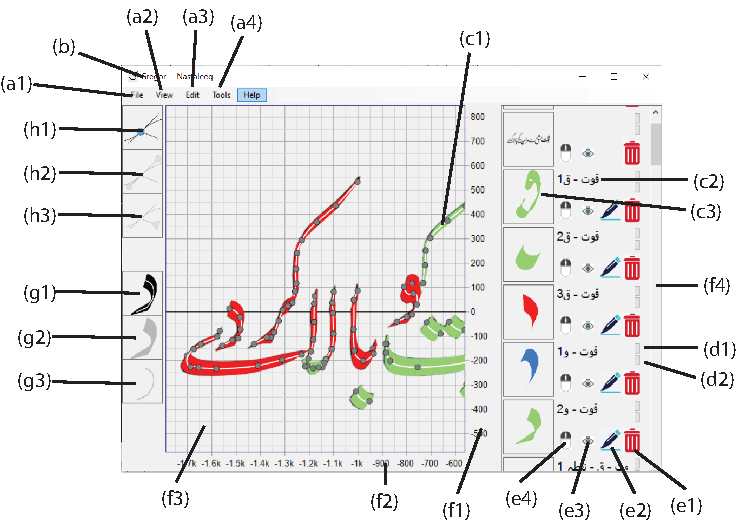
\includegraphics[width=0.9\textwidth]{GregorInterface.pdf}
      \caption{(a1-a4) The main menu options: (a1) Contains the options to open, save, import, export and clear splines and background images, (a2) enlists some viewing options; the ink viewing modes, visibility different elements of the workspace, visibility of background images, opacity of the ink-marks and rendering algorithm (a3) contains options related to editing on the workspace. It has the option to change the spline editing modes, the behaviour of left click on the workspace, and whether the splines can be dragged or not. (a4) has some analysis tools. (b) is the name of the currently open document. (c) is the main view of each spline in the document, (c2) and (c3) are the name of each spline element and its thumbnail respectively. (d1) and (d2) change the vertical order (z order) of the elements. While hovering the cursor over overlapping splines, the spline with higher position in the list will receive mouse event earlier. (e1), (e2), (e3) and (e4) are used to toggle editability, change visibility, modify color and thickness and delete the respective spline curve respectively. (f1) and (f2) are x and y axis of the workspace. (f3) is the main viewport. (f4) is the list of all the splines and images in the document. (g1) switches the view mode to both spline and inkmark, (g2) changes the viewing mode to ink only. (g3) changes the viewing mode to spline only. (h1), (h2) and (h3) toggle the visibility of center of anchor, curvature handle and the twist handle of the splines.
      } \label{Fig:GregorInterface}
    \end{figure}

}
\subsection{Modifying A Spline Curve}
{
    The application opens up an empty document by default. The first path one may choose to follow is to create new splines. This is done by adding new anchors. Anchors are added by simply clicking on an empty area of the screen. It must be noted that by default, the behaviour of the left mouse click must be switched from the Edit menu or using the keyboard shortcut to enable ``Add anchors using left mouse click''. Once an anchor has been added, adding a second anchor automatically creates a spline between the previously added anchor.
    \subsubsection{Starting a New Curve}
    {
        Since each click will append an anchor at the end of to the current spline, to break the curve and start a new one, some other procedure must be adopted. This can either be done by right clicking on an empty part of the document or toggling the ``Add anchors using left mouse click'' option off and quickly using the keyboard shortcut.
    }
    \subsubsection{Appending to a Previously Active Curve}
    {
        To append anchors at the end or the beginning of a previously active spline, simple click the center point of the first or the last center of anchor of the desired curve and it will be selected. Now, every new click will append to the selected curve just like before.
    }
    \subsubsection{Adding Anchors in the Middle}
    {
        Unfortunately adding anchor amid a curve is not a possibility yet. It would require an algorithm that can compute the nearest point on a curve from the mouse position that can show where the new anchor will be added. A work-around for now is to add anchors at the beginning or the end and soft the existing anchors inward until one of them reaches the required position.
    }
    \subsubsection{Simultaneous Curve Editing While Adding New Anchors}
    {
        It is usually very convenient to add an anchor while dragging the mouse cursor at the same time. This way, the software first adds an anchor just like it should on a mouse click but by dragging the cursor, instead of dragging the center of the newly added anchor, it drags the respective curvature handle instead. Creating new long strokes is very convenient this way. Please note that for this trick, the viewing mode must be showing the curve and both the centers and curvatures handles should be enabled.
    }
}
\subsection{Modifying an Ink-mark}
{
    \subsubsection{Adding an Ink-Mark}
    {
        Once a spline has been created with two or more anchors, the viewing mode can be switched to show ink and curve and the twist handle can be enabled while disabling the curvature handle. This will not convert the spline to a rotating curve unless it has been given a thickness. To change the thickness of a spline, simply click on it or the respective appearance in the document explorer as shown in Fig. \ref{Fig:AppearanceEditor} (e3). A curve appearance editor will pop up as shown in Fig. . Allowing to change both the broad edge thickness and the color of the ink-mark.

        \begin{figure}
          \centering
          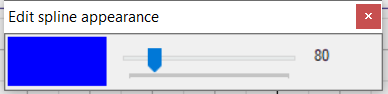
\includegraphics[width=0.3\textwidth]{appearance editor.PNG}
          \caption{The curve appearance editor lets the user modify the color and broad edge thickness of the simulated pen} \label{Fig:AppearanceEditor}
        \end{figure}
    }
    \subsubsection{Modifying the twist/rotation}
    {
        Once the Ink-mark has some thickness, it will start to show up on the viewport as well. If the rotation handles are enabled, one can start dragging each rotation handle to start twisting the curve. The artist usually continuously switches between ink and curvature handles to keep modifying the final spline until they are satisfied with the final ink-marks.
    }
}
\subsection{Using Images}
{
    Images can be imported to an existing workspace by simply selecting the menu option File > Import > Image. One can choose to import an image directly from an image file or the clipboard if the user has already copied an image using a graphics editor like a photoshop or Microsoft Paint. To view it, the background images must also be enabled from the Edit menu. Once the image is visible, the user can select a discrete handle at the middle of the image to change the placement and an anchor at the top right corner to change the size, aspect ratio, mirroring and rotation of the image.
}
\subsection{Using the Document Explorer}
{
    In addition to shoing up in the viewport, all the images and splines also appear in the document explorer as shown in Fig. \ref{Fig:GregorInterface} (f4). Each item is represented by a multi-option control which shows some controls associated with the respective item.
    \begin{itemize}
      \item Fig. \ref{Fig:GregorInterface}(c3) is a normalized thumbnail of the respective item.
      \item One can change the name of each item using Fig. \ref{Fig:GregorInterface}(c2) which can come handy while dealing with multiple items which may look similar.
      \item (e1) will delete the respective item
      \item (e2) pops up the appearance menu of the respective curve
      \item (e3) toggles the visibility of the respective item
      \item (e4) toggles the editability of an item. A Disabled item can be viewed but not interacted with.
      \item (d1) and (d2) change the order of the z-order items in a document. A simple trick while moving an item in a very long list of items is to click once on the required move button and then instead of finding the relocated button again and clicking on it again, one can now choose to press the space bar or the enter button on the keyboard which will press the button again no matter where-ever it is.
    \end{itemize}

}
\subsection{Save, Load, Export}
{
    Once the user is satisfied with the artwork, they can save it using the File menu. Once saved, the user can save any further changes to the same file by simply using the well known save command ``Control + S'' or by using the Save option from the menu again. Once saved, the file can either be opened by using the Open option in the File menu or using the windows explorer. The saved files use an extension ``rbs''. The windows usually does not recognize this extension and will thus present a list of typical applications that can open it. Choose to browse for a custom application and point to the Gregor executable. The windows will not only open the file in Gregor but also remember this choice to open rbs files in the future.

    In addition to opening a file, a user can choose to import the curves contained in a file into an existing workspace, No current items will be cleared while importing a file.

    \subsubsection{Exporting Images}
    {
        Since the curves are vector data, one may still need to export this vector into a rasterized image to be used in various circumstances. A user can export the workspace in a pixel depth of their choice using the export option in the File menu. The export window as shown in Fig. \ref{Fig:ExportMenu} presents several options
        \begin{itemize}
          \item User can control whether to include the anchors and spline curves in the render
          \item The background images can also be exported alongwith the splines.
          \item A uniform color can be selected for the exported splines.
          \item The user can also specify the rendering algorithm for the ink-mark.
          \item Last but not the least, the user can specify a pixel density. By default, each unit on the grid will be considered one pixel. Specifying a pixel density of $100$~DPU specifies to generate one hundred pixels between one unit on the grid. It must be noted that while using too dense or too large images, the application might succumb to the memory load of the procedure. So it is wise to always save the data before attempting to export an image.
        \end{itemize}

        \begin{figure}
          \centering
          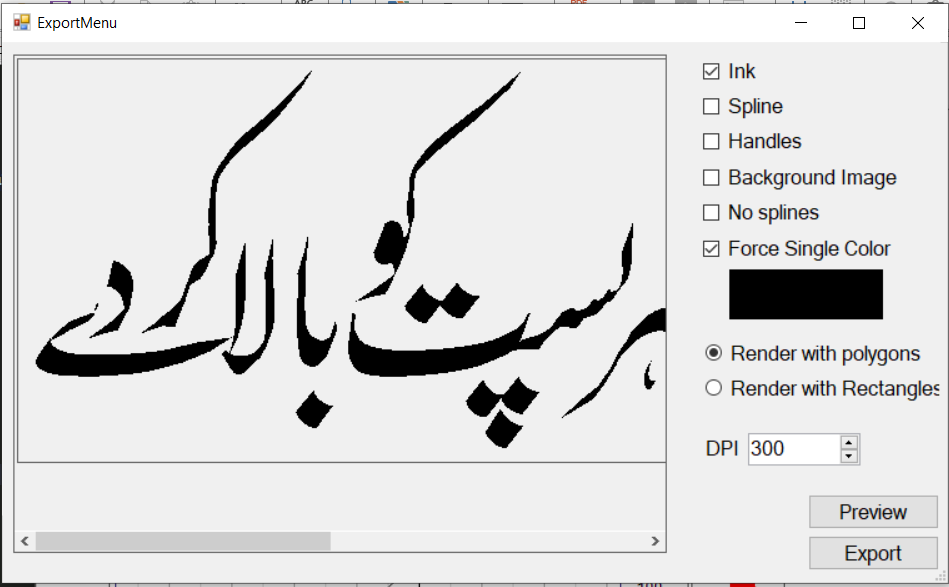
\includegraphics[width=0.9\textwidth]{ExportMenu.PNG}
          \caption{The curve appearance editor lets the user modify the color and broad edge thickness of the simulated pen} \label{Fig:ExportMenu}
        \end{figure}
    }
    \subsubsection{The File Format}
    {
        Gregor uses Microsoft XML format to save data. XML is primarily used to save text data. To pack images in it, the image is first converted into a hexadecimal list of byte data and represented as a very long string. It may inconvenience the user if they try to open it using a simple text editor which will show thousands of lines of gibberish hexadecimal bytes. One way to open the file as text is to open using an advanced raw text editor like Notepad++ or Sublime Text. These editors have the provision to collapse a certain node of an XML document, making the rest of the data more readable.
    }
}
\subsection{Short-keys}
{
    The most common keyboard shortcuts can be viewed in Table \ref{Table:Keyboardshortcuts}.
}
\subsection{Analysis Tools}
{
}
\subsection{Development}
\subsubsection{Code Organization}
\subsubsection{The BezierBoard Class}
\subsubsection{RBSPoint}
\subsubsection{Spline Elements}
\subsubsection{Miscellaneous Helper classes and form}
\subsubsection{Areas needing Improvement}

\clearpage
\section{Drogon -- The Robot Simulator}\label{Chapter:Drogon}
{
    \subsection{Introduction}

    To effectively analyze and verify the proposed solutions, a real robot was needed. Unfortunately with the COVID-19 situation, making a real robot became almost impossible with all the supply shortages and supply chain disturbances. Simulating the manipulator becomes the second option in this case. Although its not a definitive answer but with careful assumptions, a simulator ca very well be used to verify the proposals.

    A lot of effort goes behind only the software design of the simulator but ironically, in the context of the research, it is only supposed to verify whether a robot could use the twisting bezier splines to mimic the hands of an artist. This is why a lot of doors are left open for further development like implementation of other kinds of manipulators and actuators and the usage of the manipulator as a control unit for an actual robot.

    On a lighter note, just like the name Gregor, \textbf{Drogon} was also taken from a fictional character in one of the George R. R. Martin's Game of thrones novels; a mighty dragon.

    \subsubsection{The Requirements}
    Another problem was finding the best simulator to carry out the task. With no earlier training in simulators but a years of experience in programming, I decided to program an in-vitro simulator. The simulator was required to posses some important features and requirements.

    \textbf{The Simulator:}
    \begin{itemize}
      \item Simulate the position and links of the manipulator in discrete time domain.
      \item Simulate the output motors and actuators
      \item PID controllers
      \item Simulate the effect of gravity
      \item Angular and linear momentum
    \end{itemize}

    \textbf{Analysis Tools:}
    \begin{itemize}
      \item $3$~D visualizer
      \item Plotting
      \item Workspace optimizer
      \item Export data for further analysis
      \item Path planner
      \item Manual motor control
      \item Manual end effector control
      \item Machine codes parser
    \end{itemize}

    Out of all these features, there were some that could not be completed or had to be skipped given the scope of the work. Since one may be very tempted to code them or even use them, the doors to implement them are open in the code. The features are as following:
    \begin{itemize}
      \item PID controller (partly implemented)
      \item Linear and angular momentum (partly implemented)
      \item Machine code parser
    \end{itemize}

    Comprehensiveness is the core attribute of Drogon. It provides, under one screen, the flexibility to introduce an elementary change in the design, like, the maximum speed of an actuator and directly observe the consequences on all of the analysis tools. One can choose to programmatically or manually signal an actuator to move in a particular direction and position, and visualize the outcome in a $3$D preview window. It also integrates with Gregor to support the live editing and visualization of rotating bezier spline curves

    Besides comprehensiveness, our design tool offers a set of powerful analysis tools which enabled us to solve complex robot maneuvers and optimize the solution. Performing mechanical simulation with simplified real world constraints, $3$D live preview of the moving robot, work-space optimizer, $2$D art drawing, investigating the actuator velocity in continuous and discrete demain are some of the tools we used for optimization in our design.

    Since the tool is based on in-vitro coding, it can be taught to easily integrate with and inside Microcontrollers to practically , Proteus and SolidEdge to give more design flexibility.

    \subsection{The working principal}
    In this section we discuss the working principals of different aspects of the simulator.

    \subsubsection{Simulation}
    The simulator used in this work is designed from scratch. It is highly customizable in terms of coding and usage. In one configuration it can simulate a manipulator based on steppers motors. This way, the complexity of implementing the effect of gravitational and reactional forces on each actuator. In another configuration, it can simulate actuators with a limited output power, torque/force, response time and even a feedback mechanism making them essentially servo actuators. Not all of the actuators have to this way and the governing limits can also be changed at run-time. Just like the first one, in this configuration too, it first uses forward kinematics of the robot to find out the required position of its actuators to achieve a particular end-effector position and orientation. Unlike stepper motors that can just take a required number of steps in a limited time to achieve a certain position regardless of the load it has to carry, for a servo actuator, the simulator has to calculate the gravitational loads on individual links and propagate the forces and torques to individual actuator. The controller of the actuator is, in parallel, deciding how much output it must produce. Once the simulator has both the forces on each joint, it can calculate the accelerations. And once the accelerations are calculated, it only needs to be integrated with each \emph{tick} of the simulator to yield velocity and position of the actuator. At this point, it may become quite clear that implementing the gyroscopic effects of the links become quite a challenge. Since the robot being analyzed is not supposed to be working at high speeds and loads, the error caused by ignoring this effect in approximation would be negligible.

    \subsubsection{Motor controller}
    One can choose to use either a stepper motor or a DC servo on every joint. In case of stepper motors, one can configure:
    \begin{itemize}
      \item number of steps per revolution, and
      \item minimum step time.
    \end{itemize}
    In this case the simulator assumes:
    \begin{itemize}
      \item the step time remains the same regardless of the motor speed, and
      \item the motor can take a step regardless of the applied load.
    \end{itemize}
    While in case of a servo motor one can configure:
    \begin{itemize}
      \item the maximum input electrical power,
      \item the maximum torque,
      \item maximum idle acceleration,
      \item maximum velocity, and
      \item the \emph{P}, \emph{I} and \emph{D} parameters of the controller.
    \end{itemize}
    In this case, the simulator assumes that:
    \begin{itemize}
      \item the motor are $100$~% energy efficient,
      \item they are weightless, as in they are installed in the base of the robot with mechanical links transferring the power through the arm,
      \item at a constant power, the torque reduces inversely with speed ($Power = torque \times speed$), and
      \item the PID controllers operate independently.
    \end{itemize}

    Moreover, the PID controllers work on a very simple equation
    Later on, it was discovered that implementing simple PID controllers that take the required position as reference were not very effective. So the actuators are kept as stepper motors by default and can be changed to servo motors. Work is still needed to either fine tune the PID controllers or even run them on a more powerful controller.

    More details on the working principles of the simulator will be discussed in later chapters. Also, the installation and usage of the tool is described in detail in Appendix B.

    \subsubsection{Workspace}
    The workspace contains a spherical manipulator as discussed in chapter \ref{chapter2}. The simulator considers the robot fixed on a horizontal surface at the origin $(0, 0, 0)$ with the first link along the vertical axis.

    \subsection{About the Tools}

    An shape independent model of the robot under simulation can be visualized in real time using ``$3D$ Animation'' tool as seen in Fig. \ref{Fig3D}. The ``Robot Feet Position'' tool gives a superior insight on the stability of the robot. It can be seen in Fig. 1A(e) that the center of gravity plot can help optimize the motion where stability is a concern. Using the trajectory of the center of the robot in the global frame of reference can help determine the most efficient actuator movements which can be used to displace the robot from a specific position. Screen shots of the plot produced using the ``Top Trajectory'' tool can be seen in Fig. 1A(d).


        \begin{figure}
          \centering
          \includegraphics[width=0.7\textwidth]{3D.png}
          \caption{A screenshot of the $3$D representation tool. The blue sphere under the end effector shows the target given to the robot.
          } \label{Fig3D}
        \end{figure}

    All of the tools can output in real time. The robot configuration and other parameters change with time, producing animations which make it easier to decipher the underlying information.

    \subsection{Workspace Optimization}
    The workspace optimizer allows to simulate the robot solution recursively through discrete sections of the defined workspace and evaluates the degrees of freedom the robot has  specific parts of the workspace. It then colors the segments to give a more clear idea of the robot workspace. The user can then modify the robot and see, in-result, the change in the workspace. A typical output of the workspace is show in Fig.

        \begin{figure}
          \centering
          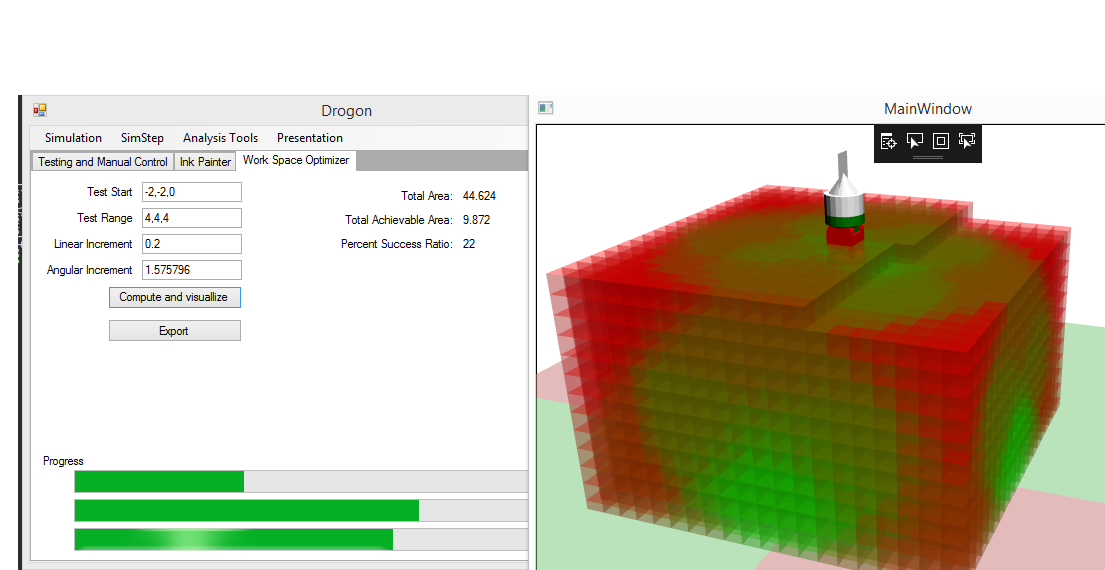
\includegraphics[width=0.9\textwidth]{WorkSpaceOptimer.png}
          \caption{The workspace is coded in colors. Purely green blocks represent a point where the robot has all of the degrees of freedom and the slightly red blocks indicate the parts where robot starts to loose one or more degrees of freedom.
          } \label{FigWorkspace}
        \end{figure}
    \subsection{Script Path Planner}
    As already mentioned, I've included a tool to construct bezier rotation splines in the tool which can serialize the data in computer files and also load from existing files. A screenshot can be seen in Fig.

        \begin{figure}
          \centering
          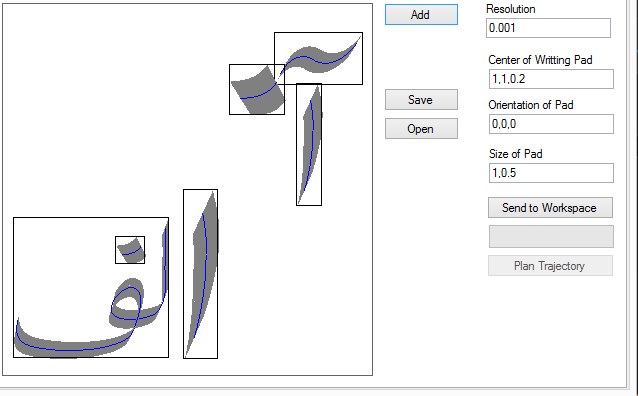
\includegraphics[width=0.9\textwidth]{SctiptEditor.png}
          \caption{The script maker can manage multiple splines and render robot trajectory according to the user resolution requirement.
          } \label{FigWorkspace}
        \end{figure}
    \subsection{Script Motion Simulator}
    Once the script is constructed using the script maker, it can be transported to the workspace in any orientation. The robot then plans how to make the required maneuvers and sibilates the behaviour. A screenshot of a robot writting a script can be seen in figure \ref{FigScriptMotion}
        \begin{figure}
          \centering
          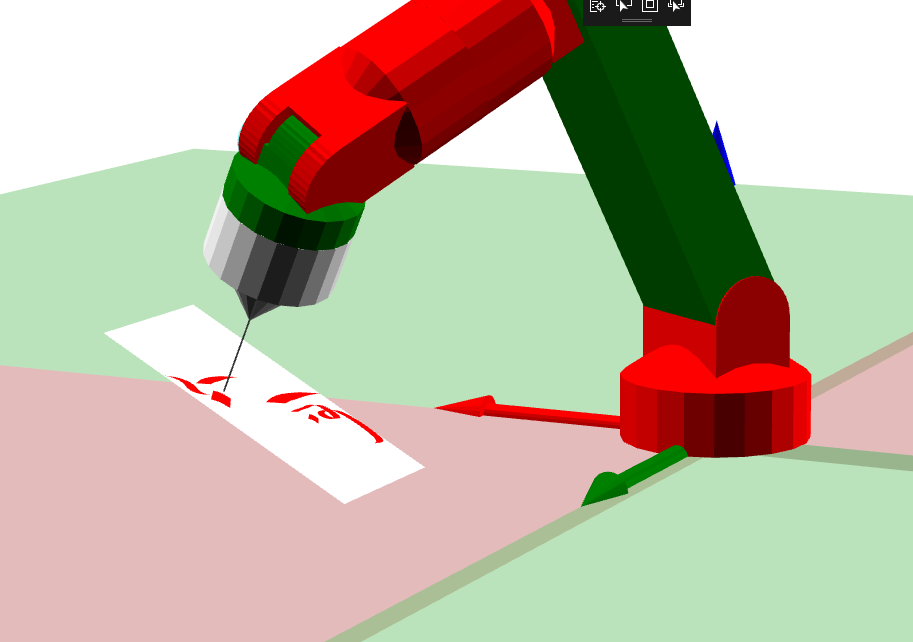
\includegraphics[width=0.9\textwidth]{writting.PNG}
          \caption{Robot writting on a slanted plane.
          } \label{FigScriptMotion}
        \end{figure}
}
\clearpage 
\end{document} 